% !TEX program = xelatex
% Cards format — auto-generated from keymaps.tex by cards-convert.mjs
\documentclass[11pt]{article}

\usepackage{fontspec}
\usepackage{unicode-math}
% Latin Modern has NO Cyrillic glyphs. STIX Two Text is a Latin-Modern-
% adjacent serif with full Cyrillic that ships on macOS AND in TeX Live,
% so the Russian cards render identically on macOS and the oven's Linux
% xelatex. Mono stays Latin Modern (only used for Latin technical text).
\setmainfont{STIX Two Text}
\setsansfont{STIX Two Text}
\setmonofont{lmmono10-regular.otf}[Scale=0.88,
  BoldFont=lmmonolt10-bold.otf,
  ItalicFont=lmmono10-italic.otf,
]


\usepackage{graphicx}
\graphicspath{{./}{figures/}}
\usepackage{booktabs}
\usepackage{tabularx}
\usepackage{adjustbox}
\usepackage{ragged2e}
\usepackage{microtype}
\usepackage{natbib}



\makeatletter
\def\input@path{{../}}
\makeatother
\usepackage{ac-paper-cards}

% The cards package defines \acbold from the Latin-only YWFT display face
% and uses it for section titles and the index. YWFT has no Cyrillic, so
% redefine \acbold to the Cyrillic-capable serif main font (bold) — this
% de-tofus every section header and the index card title.
\renewcommand{\acbold}{\rmfamily\bfseries}

% Extra commands from base paper
\newcommand{\dmn}[2]{\textcolor{#1}{\textbf{#2}}}
\newcommand{\qrc}[1]{\raisebox{\dimexpr-0.5\height+0.8ex\relax}{\includegraphics[height=0.74cm]{figures/qr/#1.png}}}
\newcommand{\klang}[2]{\href{https://papers.aesthetic.computer/keymaps-social-software-26-arxiv-cards#2.pdf}{\color{acgray}#1}}
\newcommand{\klanghere}[1]{{\bfseries\color{acpink}#1}}
\newcommand{\klangsep}{{\color{acgray!60}\,\textperiodcentered\,}}
\definecolor{keyfill}{RGB}{248,248,250}
\definecolor{keystroke}{RGB}{160,156,170}
\definecolor{keymapped}{RGB}{180,72,135}
\definecolor{keysharp}{RGB}{52,52,64}
\definecolor{acblue}{RGB}{42,100,212}
\definecolor{acgreen}{RGB}{42,154,58}
\definecolor{acorange}{RGB}{216,120,0}

% Carried from keymaps.tex: macros/packages cards-convert does not extract
% (\key/\keys live inside \makeatletter; the version stamp + colored-table
% and figure-caption commands come from the grown source paper).
\usepackage{tikz}
\usetikzlibrary{calc,positioning,shapes.geometric,arrows.meta}
\usepackage{caption}
\usepackage{colortbl}
% \ac/\acdot already come from ac-paper-cards. Carry the keycap/hex tikz
% styles the figures use (cards-convert does not extract \tikzset).
\tikzset{
 kcap/.style={draw=keystroke, fill=keyfill, rounded corners=0.6pt,
        minimum width=0.34cm, minimum height=0.34cm,
        inner sep=0pt, font=\scriptsize\sffamily},
 kcap mapped/.style={kcap, fill=keymapped!18, draw=keymapped!60,
            text=keymapped!90},
 kcap sharp/.style={kcap, fill=keysharp, draw=keysharp,
           text=white, font=\scriptsize\sffamily\bfseries},
 hexkey/.style={regular polygon, regular polygon sides=6,
         draw=keystroke, fill=keyfill, rounded corners=0pt,
         minimum size=0.55cm, inner sep=0pt,
         font=\tiny\sffamily},
 hexkey mapped/.style={hexkey, fill=keymapped!22, draw=keymapped!70,
             text=keymapped!90},
}
\DeclareRobustCommand{\key}[1]{\tikz[baseline=(k.base)]{%
 \node[fill=keystroke, rounded corners=1.3pt, inner xsep=2.4pt,
    inner ysep=1.9pt, anchor=base, yshift=-1.2pt] at (0,0)
  {\footnotesize\ttfamily\bfseries\vphantom{A}\phantom{#1}};
 \node[draw=keystroke, line width=0.4pt, fill=keyfill,
    rounded corners=1.3pt, inner xsep=2.4pt, inner ysep=1.9pt,
    anchor=base] (k) at (0,0)
  {\footnotesize\ttfamily\bfseries\vphantom{A}#1};}}
\makeatletter
\DeclareRobustCommand{\keys}[1]{{\def\sep{}\@for\kk:=#1\do{\sep\key{\kk}\def\sep{\,}}}}
\makeatother
\InputIfFileExists{version}{}{%
 \providecommand{\paperhash}{dev}\providecommand{\paperrev}{?}}
\InputIfFileExists{history}{}{\providecommand{\paperhistory}{}}

\hypersetup{
  pdftitle={Раскладки как социальное ПО: версионируемые виртуальные объекты через общественный договор},
}

\renewcommand{\acpdfbase}{keymaps-social-software-26-arxiv}
\begin{document}

% ============================================================
% TITLE CARD
% ============================================================
\thispagestyle{empty}
\vspace*{\fill}
\begin{center}
\href{https://papers.aesthetic.computer}{
\includegraphics[height=9em]{pals}}\par\vspace{0.1em}
% YWFT display face is Latin-only; the Russian title uses the serif main
% font in bold so it renders rather than dropping to tofu.
{\rmfamily\bfseries\fontsize{18pt}{22pt}\selectfont\color{acdark} Раскладки как социальное ПО}\par
\vspace{0.1em}
\vspace{0.3em}
{\normalsize\color{cyan!70!blue}\href{https://prompt.ac/@jeffrey}{\textbf{@jeffrey}}}\par
{\small\color{acgray} Aesthetic.Computer}\par
{\small\color{acgray} ORCID: \href{https://orcid.org/0009-0007-4460-4913}{0009-0007-4460-4913}}\par
\vspace{0.4em}
\rule{0.5\textwidth}{0.5pt}\par
\vspace{0.15em}
\colorbox{yellow!60}{\small\color{red!80!black}\textbf{\textit{рабочий черновик --- не цитировать}}}\par
\vspace{0.1em}
{\footnotesize\color{acgray} Март 2026 · \href{https://github.com/whistlegraph/aesthetic-computer/commit/462fcf0c0}{462fcf0c0}}\par
\vspace{0.35em}
{\footnotesize\sffamily\klang{EN}{}\klangsep\klang{DA}{-da}\klangsep\klang{ES}{-es}\klangsep\klang{ZH}{-zh}\klangsep\klang{JA}{-ja}\klangsep\klanghere{RU}}\par
\end{center}
\vspace*{\fill}

% ============================================================
% INDEX CARD
% ============================================================
\cardindex

% ============================================================
% BODY
% ============================================================
\section{Введение: артефакт}

Рисунок~\ref{fig:notepat-keymap} --- одностраничная схема раскладки, поставляемой \texttt{notepat.com}, хроматическим клавиатурным инструментом внутри \ac{}. На схеме сверху изображена фортепианная клавиатура, снизу --- клавиатура QWERTY, а пунктирные линии соединяют их. Соединяющий принцип --- лозунг, под которым выходит проект: \emph{ноты, которые сами себя называют}. Буква QWERTY \key{C} играет C; \key{D} играет D; \key{E} играет E; и так далее вплоть до \key{B}. Верхняя октава продолжается по алфавиту (\keys{H,I,J,K,L,M,N} для $C_5$ по $B_5$). Диезы располагаются по возможности на ряд выше своей натуральной ноты, по аналогии с чёрными клавишами фортепиано (\keys{V,S,W,R,Q} для $C^\sharp\,D^\sharp\,F^\sharp\,G^\sharp\,A^\sharp$).

\begin{figure*}[t]
\centering
% Native TikZ rendering of the notepat keymap diagram (Figure 1).
% Replaces the slide-pipeline PNG so the figure matches the paper's
% other vector diagrams. Piano keyboard (with the QWERTY letter that
% plays each note) above, QWERTY keyboard below, dashed color-matched
% connectors between the naturals. No hand labels — the hand split is
% carried by the two background tints and the caption.
% Key mapping verified against fedac/native/pieces/notepat.mjs and the
% AC Native screenshot: H I J K L M N = C5..B5 alphabetically (M=A5,
% N=B5), sharps V S W R Q (lower) and T Y U O P (upper).
\begingroup
% --- notepat note colors (from slides/notepat-keymap/template.html) ---
\definecolor{ncc}{HTML}{FF3232}\definecolor{ncd}{HTML}{FFA000}%
\definecolor{nce}{HTML}{FFE600}\definecolor{ncf}{HTML}{32C832}%
\definecolor{ncg}{HTML}{3278FF}\definecolor{nca}{HTML}{8232C8}%
\definecolor{ncb}{HTML}{B450FF}%
\definecolor{nCC}{HTML}{FF2850}\definecolor{nDD}{HTML}{FFB400}%
\definecolor{nEE}{HTML}{FFFF32}\definecolor{nFF}{HTML}{32FF64}%
\definecolor{nGG}{HTML}{32C8FF}\definecolor{nAA}{HTML}{B432FF}%
\definecolor{nBB}{HTML}{FF50FF}%
\definecolor{extbg}{HTML}{FFF4D6}\definecolor{extfg}{HTML}{8A7330}%
\definecolor{extbd}{HTML}{D4C075}%
\definecolor{extbk}{HTML}{5A4818}\definecolor{extbkfg}{HTML}{F8E7A0}%
\definecolor{octbg}{HTML}{F4ECFF}\definecolor{octfg}{HTML}{6B3FC0}%
\definecolor{octbd}{HTML}{B89DF0}%
\resizebox{\textwidth}{!}{%
\begin{tikzpicture}
% --- geometry ---
% piano: 17 white keys, pitch 1.02, key 0.98 x [4.4 .. 7.5]
% qwerty: caps 0.95, pitch 1.0, rows at y = 2.30 / 1.15 / 0
\def\pw{1.02}
\def\qx{2.45}
% --- piano key macros ---
\def\pkey#1#2#3#4{\begin{scope}[shift={({#1*\pw},0)}]
  \draw[acdark, fill=white, line width=0.8pt, rounded corners=1.5pt]
    (0,4.4) rectangle (0.98,7.5);
  \fill[#4] (0.04,4.44) rectangle (0.94,4.86);
  \draw[acdark!45, line width=0.4pt] (0.04,4.86) -- (0.94,4.86);
  % letter + note name live in the band BELOW the black keys
  \node[font=\large\ttfamily\bfseries, text=acdark] at (0.49,5.34) {#2};
  \node[font=\scriptsize\ttfamily, text=acdark!80] at (0.49,5.02) {#3};
\end{scope}}
\def\pkeyext#1#2#3{\begin{scope}[shift={({#1*\pw},0)}]
  \draw[extbd, dashed, fill=extbg, fill opacity=0.55, line width=0.8pt, rounded corners=1.5pt]
    (0,4.4) rectangle (0.98,7.5);
  \node[font=\large\ttfamily\bfseries, text=extfg, opacity=0.75] at (0.49,5.34) {#2};
  \node[font=\scriptsize\ttfamily, text=extfg, opacity=0.75] at (0.49,5.02) {#3};
\end{scope}}
\def\pbkey#1#2#3{\begin{scope}[shift={({#1},0)}]
  \draw[black, fill=black!92, line width=0.8pt, rounded corners=1.2pt]
    (-0.31,5.55) rectangle (0.31,7.5);
  \node[font=\normalsize\ttfamily\bfseries, text=white] at (0,6.98) {#2};
  \node[font=\fontsize{5.5pt}{5.5pt}\selectfont\ttfamily, text=white!75!black]
    at (0,6.45) {#3};
\end{scope}}
\def\pbkeyext#1#2#3{\begin{scope}[shift={({#1},0)}]
  \draw[extbk!80!black, dashed, fill=extbk, fill opacity=0.55, line width=0.8pt, rounded corners=1.2pt]
    (-0.31,5.55) rectangle (0.31,7.5);
  \node[font=\normalsize\ttfamily\bfseries, text=extbkfg, opacity=0.8] at (0,6.98) {#2};
  \node[font=\fontsize{5.5pt}{5.5pt}\selectfont\ttfamily, text=extbkfg!80]
    at (0,6.45) {#3};
\end{scope}}
% --- qwerty cap macros ---
% mapped natural: colored fill; #5 = label color (white or dark)
\def\qcap#1#2#3#4#5#6{\begin{scope}[shift={({#1},{#2})}]
  \draw[#4, fill=#3, line width=1pt, rounded corners=2.2pt]
    (0,0) rectangle (0.95,0.95);
  \node[font=\large\ttfamily\bfseries, text=#5] at (0.475,0.475) {\strut#6};
\end{scope}}
% sharp: near-black cap, border in the sharp's note color
\def\qsharp#1#2#3#4{\begin{scope}[shift={({#1},{#2})}]
  \draw[#3, fill=black!90, line width=1.1pt, rounded corners=2.2pt]
    (0,0) rectangle (0.95,0.95);
  \node[font=\large\ttfamily\bfseries, text=white] at (0.475,0.475) {\strut#4};
\end{scope}}
\def\qext#1#2#3{\begin{scope}[shift={({#1},{#2})}]
  \draw[extbd, dashed, fill=extbg, fill opacity=0.55, line width=1pt, rounded corners=2.2pt]
    (0,0) rectangle (0.95,0.95);
  \node[font=\large\ttfamily\bfseries, text=extfg, opacity=0.75] at (0.475,0.475) {\strut#3};
\end{scope}}
\def\qextbk#1#2#3{\begin{scope}[shift={({#1},{#2})}]
  \draw[extbk!80!black, dashed, fill=extbk, fill opacity=0.55, line width=1pt, rounded corners=2.2pt]
    (0,0) rectangle (0.95,0.95);
  \node[font=\large\ttfamily\bfseries, text=extbkfg, opacity=0.75] at (0.475,0.475) {\strut#3};
\end{scope}}
\def\qghost#1#2#3{\begin{scope}[shift={({#1},{#2})}]
  \draw[black!22, dashed, line width=0.9pt, rounded corners=2.2pt]
    (0,0) rectangle (0.95,0.95);
  \node[font=\large\ttfamily, text=black!30] at (0.475,0.475) {\strut#3};
\end{scope}}
\def\qoct#1#2#3#4{\begin{scope}[shift={({#1},{#2})}]
  \draw[octbd, fill=octbg, line width=1pt, rounded corners=2.2pt]
    (0,0) rectangle (0.95,0.95);
  \node[font=\large\ttfamily\bfseries, text=octfg] at (0.475,0.55) {\strut#3};
  \node[font=\fontsize{5pt}{5pt}\selectfont\sffamily\bfseries, text=octfg!75]
    at (0.475,0.2) {#4};
\end{scope}}
% --- hand-split background tints behind the qwerty block ---
\fill[acblue!8, rounded corners=4pt] (\qx-0.25,-0.3) rectangle (\qx+6.07,3.55);
\fill[acpink!8, rounded corners=4pt] (\qx+6.07,-0.3) rectangle (\qx+12.6,3.55);
% --- connectors (drawn LAST so they compose over the keys) ---
\def\conn#1#2#3#4#5{%
  \draw[#4, dashed, line width=1.1pt, opacity=#5, line cap=round]
    ({#1*\pw+0.49},4.62) -- ({#2+0.475},{#3+0.80});
  \fill[#4, opacity=#5] ({#1*\pw+0.49},4.62) circle (0.055);
  \fill[#4, opacity=#5] ({#2+0.475},{#3+0.80}) circle (0.055);}
% --- piano: white keys ---
\pkeyext{0}{X}{B3}
\pkey{1}{C}{C4}{ncc}  \pkey{2}{D}{D4}{ncd}  \pkey{3}{E}{E4}{nce}
\pkey{4}{F}{F4}{ncf}  \pkey{5}{G}{G4}{ncg}  \pkey{6}{A}{A4}{nca}
\pkey{7}{B}{B4}{ncb}
\pkey{8}{H}{C5}{nCC}  \pkey{9}{I}{D5}{nDD}  \pkey{10}{J}{E5}{nEE}
\pkey{11}{K}{F5}{nFF} \pkey{12}{L}{G5}{nGG} \pkey{13}{M}{A5}{nAA}
\pkey{14}{N}{B5}{nBB}
\pkeyext{15}{;}{C6} \pkeyext{16}{]}{D6}
% --- piano: black keys (centered on white-key boundaries) ---
\pbkeyext{0.35}{Z}{A\#3}
\pbkey{2.04}{V}{C\#4}  \pbkey{3.06}{S}{D\#4}
\pbkey{5.10}{W}{F\#4}  \pbkey{6.12}{R}{G\#4}  \pbkey{7.14}{Q}{A\#4}
\pbkey{9.18}{T}{C\#5}  \pbkey{10.20}{Y}{D\#5}
\pbkey{12.24}{U}{F\#5} \pbkey{13.26}{O}{G\#5} \pbkey{14.28}{P}{A\#5}
\pbkeyext{16.32}{'}{C\#6}
% --- qwerty row 0 (top): Q W E R T Y U I O P [ ] ---
\qsharp{\qx+0}{2.30}{nca}{Q}
\qsharp{\qx+1}{2.30}{ncf}{W}
\qcap{\qx+2}{2.30}{nce}{nce!60!black}{black!75}{E}
\qsharp{\qx+3}{2.30}{ncg}{R}
\qsharp{\qx+4}{2.30}{nCC}{T}
\qsharp{\qx+5}{2.30}{nDD}{Y}
\qsharp{\qx+6}{2.30}{nFF}{U}
\qcap{\qx+7}{2.30}{nDD}{nDD!60!black}{white}{I}
\qsharp{\qx+8}{2.30}{nGG}{O}
\qsharp{\qx+9}{2.30}{nAA}{P}
\qghost{\qx+10}{2.30}{[}
\qext{\qx+11}{2.30}{]}
% --- qwerty row 1 (home): A S D F G H J K L ; ' ---
\qcap{\qx+0.28+0}{1.15}{nca}{nca!60!black}{white}{A}
\qsharp{\qx+0.28+1}{1.15}{ncd}{S}
\qcap{\qx+0.28+2}{1.15}{ncd}{ncd!60!black}{white}{D}
\qcap{\qx+0.28+3}{1.15}{ncf}{ncf!60!black}{white}{F}
\qcap{\qx+0.28+4}{1.15}{ncg}{ncg!60!black}{white}{G}
\qcap{\qx+0.28+5}{1.15}{nCC}{nCC!60!black}{white}{H}
\qcap{\qx+0.28+6}{1.15}{nEE}{nEE!55!black}{black!70}{J}
\qcap{\qx+0.28+7}{1.15}{nFF}{nFF!55!black}{black!60}{K}
\qcap{\qx+0.28+8}{1.15}{nGG}{nGG!55!black}{black!60}{L}
\qext{\qx+0.28+9}{1.15}{;}
\qextbk{\qx+0.28+10}{1.15}{'}
% --- qwerty row 2 (bottom): Z X C V B N M , . / ---
\qextbk{\qx+0.84+0}{0}{Z}
\qext{\qx+0.84+1}{0}{X}
\qcap{\qx+0.84+2}{0}{ncc}{ncc!60!black}{white}{C}
\qsharp{\qx+0.84+3}{0}{ncc}{V}
\qcap{\qx+0.84+4}{0}{ncb}{ncb!60!black}{white}{B}
\qcap{\qx+0.84+5}{0}{nBB}{nBB!60!black}{white}{N}
\qcap{\qx+0.84+6}{0}{nAA}{nAA!60!black}{white}{M}
\qoct{\qx+0.84+7}{0}{,}{OCT$-$}
\qoct{\qx+0.84+8}{0}{.}{OCT$+$}
\qghost{\qx+0.84+9}{0}{/}
% connectors drawn last — composed over the keys
\conn{1}{\qx+0.84+2}{0}{ncc}{0.85}      % C4 -> C (row 2)
\conn{2}{\qx+0.28+2}{1.15}{ncd}{0.65}   % D4 -> D
\conn{3}{\qx+2}{2.30}{nce!75!black}{0.55} % E4 -> E
\conn{4}{\qx+0.28+3}{1.15}{ncf}{0.50}   % F4 -> F
\conn{5}{\qx+0.28+4}{1.15}{ncg}{0.45}   % G4 -> G
\conn{6}{\qx+0.28+0}{1.15}{nca}{0.40}   % A4 -> A
\conn{7}{\qx+0.84+4}{0}{ncb}{0.35}      % B4 -> B
\conn{8}{\qx+0.28+5}{1.15}{nCC}{0.55}   % C5 -> H
\conn{9}{\qx+7}{2.30}{nDD}{0.45}        % D5 -> I
\conn{10}{\qx+0.28+6}{1.15}{nEE!70!black}{0.40} % E5 -> J
\conn{11}{\qx+0.28+7}{1.15}{nFF!80!black}{0.40} % F5 -> K
\conn{12}{\qx+0.28+8}{1.15}{nGG!80!black}{0.40} % G5 -> L
\conn{13}{\qx+0.84+6}{0}{nAA}{0.35}     % A5 -> M
\conn{14}{\qx+0.84+5}{0}{nBB}{0.32}     % B5 -> N
\end{tikzpicture}}
\endgroup

\caption{Раскладка \texttt{notepat.com}. Буква QWERTY \key{C} играет C, \key{D} играет D, ..., \key{B} играет B; верхняя октава продолжается по алфавиту (\keys{H,I,J,K,L,M,N}); диезы по возможности располагаются над своей натуральной нотой по аналогии с чёрными клавишами фортепиано. Двуручное разделение: нижняя октава под левой рукой (синее поле), верхняя --- под правой (розовое поле); приглушённые клавиши расширяют диапазон. Реализации: \texttt{notepat.com} (веб), AC Native OS, MenuBand (строка меню macOS), плагин Ableton (Max for Live), \texttt{babypat}.}
\label{fig:notepat-keymap}
\end{figure*}

Эта схема и есть артефакт. Она мала. Она не содержит кода. Это не бинарник, не сервис, не среда исполнения. Это таблица. И тем не менее из всех компонентов, составляющих \texttt{notepat.com}, именно таблица --- та, что путешествует, та, которую всякий, кто играет на производном от notepat инструменте в вебе, AC Native, строке меню macOS, Max for Live или телефонном приложении, должен знать и принимать. Таблица --- это то, что делает \texttt{notepat.com} \emph{самим собой} поверх разных субстратов, --- и то же верно для инструментов вообще: раскладка --- это то, что придаёт инструменту, \texttt{notepat.com} или любому другому, его идентичность на каждой поверхности, его несущей.

Эта статья о таком роде таблиц. Я буду называть её \emph{раскладкой} и буду утверждать, что раскладки образуют категорию вычислительных артефактов, которую стандартная рамка академических исследований вычислений --- рамка, организованная вокруг бинарников, проектов и лицензий, --- не способна различить. Категория не мала. Среди её прочих членов --- сама раскладка QWERTY, раскладка Dvorak, Colemak и его форки, изоморфная нотная раскладка Wicki--Hayden, хроматически-лестничное отображение QWERTY-фортепиано, общее для каждой крупной цифровой рабочей станции, нотация Сингмастера для алгоритмов кубика Рубика~\citep{singmaster1981notes}, Нэшвиллская числовая система~\citep{matthews1984nashville}, стенотеория Plover~\citep{knight2010plover}, нумпад-нотация файтингов, колесо Camelot~\citep{davis1991camelot} и комбинации клавиш Vim, среди многих других.

Я буду называть эту категорию \emph{социальным ПО}, и название несёт сразу две линии. Первая --- термин Ширки 2003 года~\citep{shirky2003etech,allen2004socialsoftware}: там, где Ширки и его современники использовали «социальное ПО» для обозначения \emph{ПО, опосредующего социальное взаимодействие} --- форумов, вики, чат-систем, --- я использую его для обозначения \emph{ПО, чьё существование \textbf{есть} социальное согласие}. Это прочтение --- каламбур, параллельный и немного неожиданный. Вторая линия ближе, и это контекст, внутри которого написана эта статья: \emph{Social Software} --- инициатива в UCLA Design\,\textbar\,Media Arts под руководством Lauren Lee McCarthy и Casey Reas~\citep{sosoft_info}, которая определяет свой предмет как «любую систему, организующую поведение, координирующую людей или структурирующую взаимодействие»; \emph{Auto} Маккарти, перформанс, разыгранный внутри автономного автомобиля, есть социальное ПО ровно в этом смысле~\citep{mccarthy2026auto}. Я пишу как приглашённый художник во втором цикле инициативы, \emph{Scores for Social Software}, под руководством Риса~\citep{reas2026scores}, который прочитывает \emph{партитуру} --- инструкцию Флюксуса, \emph{Notations} Кейджа и Ноулз, \emph{do it} Обриста~\citep{cage1969notations,obrist1997doit} --- как способ хореографии событий во времени посредством текста, диаграмм или иных форм инструкции. Раскладка --- именно такая партитура: небольшая инструктивная таблица, которая хореографирует руки, распространяется как текст и диаграмма и организует поведение всякого, кто её принимает. У раскладки нет компилятора, нет среды исполнения, нет организации-сопровождающего и редко --- финансового механизма за ней. Она существует потому, что достаточное число людей решили действовать так, будто она существует. Она сохраняется потому, что пользователи требуют межбинарной совместимости с ней. Когда эта совместимость нарушается, пользователи замечают; когда она сохраняется, раскладка распространяется дальше.

Статья развивается в семи движениях. \textsection\ref{sec:category} формулирует проблему категории: раскладки имеют форму ПО, но не суть ПО, и ось «открытый код/проприетарный» их не различает. \textsection\ref{sec:lineage1}--\ref{sec:lineage2} прослеживают две линии изобретения раскладок --- линию «от пишущей машинки к компьютеру» (Шоулз, Dvorak, Colemak) и линию музыкальных инструментов (Янко, Wicki--Hayden, современные гекс-изоморфные контроллеры). \textsection\ref{sec:daw} рассматривает доминирующий современный случай: хроматически-лестничную раскладку QWERTY-фортепиано, которую Ableton, Logic, GarageBand и FL Studio все поставляют по умолчанию, --- никому не принадлежащую конвенцию, которую никто не спроектировал, никто не сопровождает и все реализуют. \textsection\ref{sec:notepat} прочитывает раскладку «ноты, которые сами себя называют» от \texttt{notepat.com} как намеренное вмешательство против этого предшественника: не наследование, не форк, а конкурирующее предложение о том, как должна выглядеть таблица, --- и проводит черту между тональным договором, который должна нести каждая реализация, и расширенным исполнительским слоем, который каждый субстрат отращивает сам. \textsection\ref{sec:notation} вводит поверхность нотации: у каждой раскладки есть текстовая форма, в которой путешествует её употребление, и нотация часто оказывается более долговечной половиной артефакта --- структурное утверждение, где Vim служит каноническим положительным случаем, а DAW-лестница --- отрицательным. \textsection\ref{sec:corollaries} каталогизирует более широкий род, показывая, что отображения ввода, нотационные системы и категориальные ярлыки разделяют общий социально-программный паттерн. \textsection\ref{sec:lialina} прочитывает корпус свидетельств сквозь «Тьюринг-полного пользователя» Лиалиной, утверждая, что раскладки --- эмпирическое тело её тезиса о том, что пользователи суть программисты в ожидании. \textsection\ref{sec:design} завершает тем, чего это требует от дизайнеров: поставлять раскладку как полноправный объект --- читаемый, экспортируемый, форкаемый --- и нотацию вместе с ней.

\section{Проблема категории}
\label{sec:category}

Раскладка --- небольшая декларативная таблица. Минимальная форма --- список пар: \emph{(событие-физической-клавиши, семантический-вывод)}. Раскладка QWERTY --- таблица, сопоставляющая позиции клавиш с буквами; раскладка Dvorak переназначает те же позиции иному набору букв; хроматически-лестничное отображение QWERTY-фортепиано сопоставляет каждой клавише номер MIDI-ноты; кубическая нотация Сингмастера сопоставляет каждому ярлыку грани вращательный оператор. Во всех случаях артефакт --- именно таблица. Бинарник, потребляющий таблицу, взаимозаменяем.

Это затрудняет размещение раскладок внутри господствующих рамок академических исследований вычислений. Ось «открытый код/проприетарный»~\citep{galloway2004protocol} сортирует ПО по правовому статусу его исходного кода. У раскладки нет исходного кода --- это таблица, а не программа. Ось платформенных исследований~\citep{nieborg2018platformization} сортирует ПО по платформе, на которой оно стоит. Раскладка стоит на \emph{каждой} платформе, потребляющей её форму. Ось теории форматов~\citep{sterne2012mp3} сортирует ПО по спецификации, которую оно реализует. У раскладки редко есть спецификация; у хроматически-лестничного отображения QWERTY-фортепиано её нет, и тем не менее четыре крупнейшие в мире DAW все поставляют одно и то же. Ось протокола~\citep{galloway2004protocol} сортирует ПО по сетевому формату, на котором оно говорит. Раскладка --- не сетевой формат; это таблица, к которой обращаются на границе ввода.

Ближе всего подходит \emph{MP3: The Meaning of a Format} Стерна~\citep{sterne2012mp3}. Стерн утверждает, что «форматы, стандарты и инфраструктуры --- и необходимость для контента вписываться в них --- столь же центральны для коммуникации, как и ящики, которые мы зовём „медиа“». Подставьте \emph{раскладку} вместо \emph{формата}, и бóльшая часть его аппарата переносится. Но у форматов есть спецификации (RFC, документы ISO, эталонные реализации). У раскладок обычно нет. Хроматически-лестничное отображение QWERTY-фортепиано реализовано в Ableton Live, Logic Pro, GarageBand и FL Studio~\citep{ableton_musical_typing,apple_logic_musicaltyping,imageline_typing_piano}, ни разу не будучи записанным в обязывающей спецификации. Оно существует потому, что четыре реализации согласны, а четыре реализации согласны потому, что всякий, кто выучил одну, ожидает, что следующая будет такой же.

\emph{Sorting Things Out} Боукера и Стар~\citep{bowker1999sorting} трактует классификации и стандарты как социально-политические объекты, чья устойчивость социологична, а не технична. Раскладка --- классификация: она сортирует физические вводы в семантические категории. \emph{Граничный объект} Стар и Гризмера~\citep{star1989boundary} схватывает другой аспект: раскладки опосредуют между сообществами практики (машинистка и программист; пианист и пользователь DAW; кубер и решающий кубик), не принадлежа полностью ни одному. \emph{Этнография инфраструктуры} Стар~\citep{star1999ethnography} схватывает третий: раскладки скучны, значимы и по большей части невидимы для тех, кто от них зависит.

То, что мы хотим назвать, --- это конъюнкция этих признаков: небольшая таблица, которая есть классификация (Боукер и Стар), граничный объект (Стар и Гризмер), инфраструктура (Стар) и формат (Стерн), --- но не есть ни одно из этого по отдельности. Я предлагаю \emph{социальное ПО} для этой конъюнкции. Термин теперь несёт три прочтения, и все они реальны. В 2003 году он назвал \emph{ПО для социальности} (Ширки); в UCLA сегодня он называет \emph{любую систему, организующую поведение, координирующую людей или структурирующую взаимодействие} (Маккарти и Рис~\citep{sosoft_info}); эта статья предлагает, чтобы он называл также \emph{ПО социального согласия}. Раскладка --- третье прочтение напрямую, --- а прочитанная как партитура, хореографирующая руки всякого, кто её принимает, она помещается прямо внутрь второго.

\section{Линия I: раскладки клавиатуры}
\label{sec:lineage1}

Самый ранний устойчивый пример раскладки-как-социального-ПО --- сама раскладка QWERTY. Кристофер Лэтэм Шоулз запатентовал раннюю пишущую машинку вместе с Карлосом Глидденом и Сэмюэлом Сулé в 1868 году (US 79{,}265); поставляемое расположение QWERTY было окончательно оформлено внутри компании механиками Remington весной и летом 1873 года как инженерно-производственное решение и \emph{никогда не было запатентовано}~\citep{yasuoka2011prehistory}. Стандартный фольклорный рассказ приписывает раскладку механике против заклинивания; архивная работа Ясуоки и Ясуоки помещает её в практику транскрипции телеграфистов, которым нужно было печатать азбуку Морзе в реальном времени. Так или иначе, устойчивость раскладки социологична: это основополагающий эмпирический случай экономики зависимости от пути~\citep{david1985qwerty,arthur1989competing}, с контртрадицией, утверждающей, что доминирование преувеличено~\citep{liebowitz1990fable}. Спор Дэвида и Либовица --- первичная сцена для трактовки отображения ввода как объекта, чья устойчивость есть эмпирический вопрос о социальном принятии, а не выводимое следствие технического превосходства.

Огест Дворак и Уильям Дили запатентовали упрощённую клавиатуру Dvorak в 1936 году (US 2{,}040{,}248). Они утверждали, что она быстрее, менее утомительна и педагогически рациональнее QWERTY. Она распространялась неравномерно: ВМС США приняли её в исследованиях во время Второй мировой войны; Apple IIc поставлялся с переключателем Dvorak; современные операционные системы все поставляют Dvorak как выбираемую раскладку; и небольшое, но устойчивое сообщество пользователей применяет её десятилетиями. Workman~\citep{bucao2010workman}, Colemak~\citep{coleman2006colemak} и экосистема форков после 2010 года (Colemak-DH, Halmak, Norman) составляют третье поколение. Ни у одной из этих раскладок нет организации-сопровождающего. Ни у одной нет дохода. Все они --- версионируемые виртуальные объекты, распространяющиеся через форумы, репозитории GitHub и файлы раскладок операционных систем. Клавиатура Maltron~\citep{malt1977keyboard} добавила аппаратно сопряжённый вариант; стенотеория Plover~\citep{knight2010plover} расширила поверхность до аккордовой скорописи. Национальные раскладки (AZERTY, QWERTZ, BÉPO) участвуют в той же логике, с дополнительным поворотом формального государственного признания: французская раскладка BÉPO, спроектированная сообществом в 2005 году, была свёрнута в национальный стандарт AFNOR 2019 года --- буквально наблюдаемый переход от общественного договора к государственному.

\begin{figure}[t]
\centering
\resizebox{\columnwidth}{!}{%
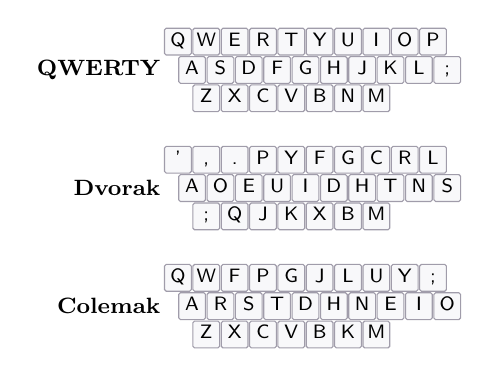
\begin{tikzpicture}
% Three keyboards stacked. Same 30 physical key positions; each layout
% reassigns the letters at those positions. Visual comparison highlights
% how a keymap is a re-binding of an unchanged physical substrate.
% Three keyboards stacked. Punctuation chars are wrapped in {} so
% TikZ's \foreach parser doesn't treat them as separators.
\foreach \layoutY/\name in {3.0/QWERTY, 1.5/Dvorak, 0.0/Colemak} {
 \node[anchor=east, font=\footnotesize\bfseries] at (-0.1, \layoutY+0.36) {\name};
}
% QWERTY rows
\foreach \l [count=\i] in {Q,W,E,R,T,Y,U,I,O,P}
 \node[kcap] at ({(\i-1)*0.36}, 3.72) {\strut\l};
\foreach \l [count=\i] in {A,S,D,F,G,H,J,K,L,{;}}
 \node[kcap] at ({(\i-1)*0.36+0.18}, 3.36) {\strut\l};
\foreach \l [count=\i] in {Z,X,C,V,B,N,M}
 \node[kcap] at ({(\i-1)*0.36+0.36}, 3.0) {\strut\l};
% Dvorak rows
\foreach \l [count=\i] in {{'},{,},{.},P,Y,F,G,C,R,L}
 \node[kcap] at ({(\i-1)*0.36}, 2.22) {\strut\l};
\foreach \l [count=\i] in {A,O,E,U,I,D,H,T,N,S}
 \node[kcap] at ({(\i-1)*0.36+0.18}, 1.86) {\strut\l};
\foreach \l [count=\i] in {{;},Q,J,K,X,B,M}
 \node[kcap] at ({(\i-1)*0.36+0.36}, 1.5) {\strut\l};
% Colemak rows
\foreach \l [count=\i] in {Q,W,F,P,G,J,L,U,Y,{;}}
 \node[kcap] at ({(\i-1)*0.36}, 0.72) {\strut\l};
\foreach \l [count=\i] in {A,R,S,T,D,H,N,E,I,O}
 \node[kcap] at ({(\i-1)*0.36+0.18}, 0.36) {\strut\l};
\foreach \l [count=\i] in {Z,X,C,V,B,K,M}
 \node[kcap] at ({(\i-1)*0.36+0.36}, 0) {\strut\l};
\end{tikzpicture}}
\caption{Три печатные раскладки над одним физическим субстратом. Каждая раскладка --- это перепривязка одних и тех же позиций клавиш к иному набору букв. QWERTY (Шоулз 1873, никогда не патентовалась), Dvorak (Dvorak и Dealey 1936, US 2{,}040{,}248), Colemak (Coleman 2006, общественное достояние). Экосистема форков после 2010 года продолжает эту линию.}
\label{fig:typing-layouts}
\end{figure}

\section{Линия II: раскладки инструментов}
\label{sec:lineage2}

Раскладки музыкальных инструментов прошли параллельную историю. Шестирядная изоморфная фортепианная клавиатура Пауля фон Янко~\citep{janko1882} была одобрена Листом и Рубинштейном, производилась Decker, Blüthner и Bösendorfer и преподавалась в консерватории Янко в Нью-Йорке. По всем социальным предпосылкам принятия она должна была заменить стандартную фортепианную клавиатуру. Этого не произошло. Известно, что сохранилось менее десяти фортепиано Янко. Случай Янко --- отрицательный полюс аргумента раскладки-как-социального-ПО: всякое условие распространения было выполнено, а распространение всё равно провалилось. Чем бы ни был социально-программный договор, он больше суммы одобрений, производителей и консерваторий.

Обобщённая клавиатура Р.\ Х.\ М.\ Босанке~\citep{bosanquet1875generalized} была энгармонической фисгармонией с 53-равным делением октавы (53-EDO) и органом 1875 года в 48-нотном схизматическом и четвертькоммном среднетоновом строе, продемонстрированным Южно-Кенсингтонскому музею в 1876 году. Это предок по сути всякого современного изоморфного контроллера. Каспар Wicki запатентовал изоморфную нотную раскладку для бандонеона в 1896 году~\citep{wicki1896}; Brian Hayden, играющий на концертине, независимо переизобрёл и перепатентовал по сути ту же раскладку в 1986 году. Двойное изобретение с разницей в девяносто лет само по себе есть аргумент: раскладка имеет характер \emph{открытия}, объекта, который повторяется потому, что лежащая в основе структура музыки делает его полезным, а не потому, что это уникальный культурный артефакт.

\begin{figure}[t]
\centering
\resizebox{0.88\columnwidth}{!}{%
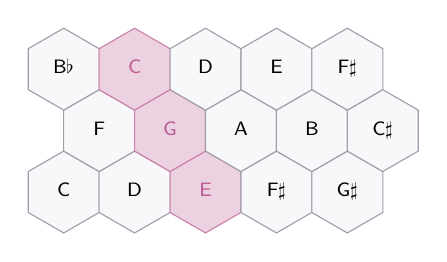
\begin{tikzpicture}
% Compact Wicki-Hayden-style hex schematic. Same-row neighbors
% differ by a whole tone; up-and-right neighbors differ by a P4.
% C major triad (C-E-G) highlighted; the same shape transposes to
% any key by translation across the surface ("isomorphism" claim).
% Hexes are EXPLICIT PATHS, not regular-polygon nodes — TikZ node
% sizing breaks the lattice. Pointy-top hexagon, circumradius R:
% width = sqrt(3)R, height = 2R. Tessellation: horizontal pitch =
% sqrt(3)R, row step = 1.5R, odd-row offset = sqrt(3)R/2.
\def\R{0.52}
\def\hexn#1#2#3{\begin{scope}[shift={(#1,#2)}]
 \draw[keystroke, fill=keyfill]
  (30:\R) -- (90:\R) -- (150:\R) -- (210:\R) -- (270:\R) -- (330:\R) -- cycle;
 \node[font=\scriptsize\sffamily, inner sep=0pt] at (0,0) {\strut#3};
\end{scope}}
\def\hexm#1#2#3{\begin{scope}[shift={(#1,#2)}]
 \draw[keymapped!70, fill=keymapped!25]
  (30:\R) -- (90:\R) -- (150:\R) -- (210:\R) -- (270:\R) -- (330:\R) -- cycle;
 \node[font=\scriptsize\sffamily, text=keymapped!90, inner sep=0pt] at (0,0) {\strut#3};
\end{scope}}
\def\hp{0.9006}  % horizontal pitch (sqrt(3) * R)
\def\vp{0.78}   % vertical pitch (1.5 * R)
\def\offx{0.4503} % horizontal offset for alternate rows (hp / 2)
% Row 0 (bottom)
\hexn{0}{0}{C}
\hexn{\hp}{0}{D}
\hexm{2*\hp}{0}{E}
\hexn{3*\hp}{0}{F$\sharp$}
\hexn{4*\hp}{0}{G$\sharp$}
% Row 1 (middle, offset)
\hexn{\offx}{\vp}{F}
\hexm{\offx + \hp}{\vp}{G}
\hexn{\offx + 2*\hp}{\vp}{A}
\hexn{\offx + 3*\hp}{\vp}{B}
\hexn{\offx + 4*\hp}{\vp}{C$\sharp$}
% Row 2 (top)
\hexn{0}{2*\vp}{B$\flat$}
\hexm{\hp}{2*\vp}{C}
\hexn{2*\hp}{2*\vp}{D}
\hexn{3*\hp}{2*\vp}{E}
\hexn{4*\hp}{2*\vp}{F$\sharp$}
\end{tikzpicture}}
\caption{Гекс-раскладка Wicki--Hayden (Wicki 1896 / Hayden 1986). Соседи по одному ряду различаются на целый тон; соседи вверх-и-вправо --- на чистую кварту. Мажорное трезвучие до ($C\,E\,G$) выделено: аккорд --- фиксированная трёхклеточная форма на поверхности, и перенос этой формы транспонирует аккорд в любую тональность. «Транспозиция есть перенос» --- центральное утверждение изоморфной клавиатуры и свойство, которым жертвует бело-чёрная асимметрия стандартного фортепиано.}
\label{fig:wicki}
\end{figure}

\begin{figure*}[t]
\centering
% Interval-signature bars (full text width). Each bar reads left to
% right as the sequence of intervals the instrument's layout steps
% through; every block is one interval, its WIDTH = its size in
% semitones and its COLOR fixed by the legend. A regular instrument
% is a row of equal blocks; an asymmetric one has a visible odd block.
\begingroup
\definecolor{iv1}{HTML}{E2574C}% m2 (1 semitone)
\definecolor{iv2}{HTML}{EE9B3A}% M2 (2)
\definecolor{iv3}{HTML}{D1A52A}% m3 (3) — darkened so white slice text reads
\definecolor{iv4}{HTML}{4FAE54}% M3 (4)
\definecolor{iv5}{HTML}{3A86D6}% P4 (5)
\definecolor{iv7}{HTML}{8A5CF6}% P5 (7)
\resizebox{\textwidth}{!}{%
\begin{tikzpicture}
\def\rad{1.55}
% \pie{xshift}{name}{deg-per-semitone}{ semitones/color/label, ... }
% Slices sweep clockwise from 12 o'clock; angle = semitones. A regular
% instrument is an even wheel; an asymmetric one has a visibly odd slice.
% list fields: semitones / fill / interval-label / note-label.
% The note sits INSIDE the slice (the actual open string, scale degree,
% or valve number); the interval name sits just outside the rim.
\def\pie#1#2#3#4{\begin{scope}[shift={(#1,0)}]
 \xdef\angA{90}
 \foreach \s/\c/\lab/\nt in {#4}{
  \pgfmathsetmacro\angB{\angA-\s*#3}
  \filldraw[fill=\c, draw=\c!55!black, line width=0.6pt]
   (0,0) -- (\angA:\rad) arc[start angle=\angA, end angle=\angB, radius=\rad] -- cycle;
  \pgfmathsetmacro\angM{(\angA+\angB)/2}
  \node[font=\large\sffamily\bfseries, text=white] at (\angM:{0.58*\rad}) {\nt};
  \node[font=\small\sffamily, text=acdark] at (\angM:{\rad+0.32}) {\lab};
  \xdef\angA{\angB}
 }
 \node[font=\normalsize\sffamily\bfseries, text=acdark] at (0,{-\rad-1.08}) {#2};
\end{scope}}
% --- legend ---
\begin{scope}[shift={(-0.4,3.15)}]
 \node[font=\small\sffamily\bfseries, text=acdark, anchor=west] at (0,0.28) {Интервал \;(угол сектора $\propto$ полутонам):};
 \def\lg#1#2#3{\draw[fill=#2, draw=#2!55!black, rounded corners=2pt] (#1,0.0) rectangle (#1+0.56,0.56);
  \node[font=\small\sffamily, text=acdark, anchor=west] at (#1+0.66,0.28) {#3};}
 \lg{7.7}{iv1}{m2}\lg{9.1}{iv2}{M2}\lg{10.5}{iv3}{m3}\lg{11.9}{iv4}{M3}\lg{13.3}{iv5}{P4}\lg{14.7}{iv7}{P5}
\end{scope}
% --- four wheels in a row ---
\pie{0}{Гитара \textperiodcentered\ EADGBE}{15}{5/iv5/P4/E, 5/iv5/P4/A, 5/iv5/P4/D, 4/iv4/M3/G, 5/iv5/P4/B}
% emphasize the guitar's lone M3 wedge (starts -135, spans 60 deg)
\draw[keymapped, line width=1.5pt]
 (0,0) -- (-135:\rad) arc[start angle=-135, end angle=-195, radius=\rad] -- cycle;
\pie{4.7}{Скрипка \textperiodcentered\ GDAE}{17.142857}{7/iv7/P5/G, 7/iv7/P5/D, 7/iv7/P5/A}
\pie{9.4}{Труба \textperiodcentered\ 3 вентиля}{60}{2/iv2/M2/1, 1/iv1/m2/2, 3/iv3/m3/3}
\pie{14.1}{Окарина \textperiodcentered\ диатоника}{30}{2/iv2/M2/C, 2/iv2/M2/D, 1/iv1/m2/E, 2/iv2/M2/F, 2/iv2/M2/G, 2/iv2/M2/A, 1/iv1/m2/B}
\end{tikzpicture}}
\endgroup
\caption{Четыре асимметричных высотных интерфейса, прочитанных как \emph{интервальные колёса}. Каждое колесо проходит по часовой стрелке через интервалы, из которых построена его раскладка; каждый сектор --- один интервал, его угол задан размером в полутонах, а цвет фиксирован легендой. Регулярный инструмент --- ровное колесо; асимметричный несёт зримо нечётный сектор. Гитара EADGBE --- кольцо чистых кварт, прерванное единожды большой терцией между G и B (обведена), --- неправильность, благодаря которой стандартные аккордовые формы ложатся под руку и под которую авторски писались фолк, блюз, джаз и рок-гитара. Скрипка --- три одинаковые чистые квинты: совершенно ровное колесо, и всё же каждая открытая струна --- иная абсолютная высота. Три вентиля трубы понижают высоту на два, один и три полутона --- все различны по замыслу, так что их комбинации достигают каждой хроматической ступени. Окарина --- собственное колесо диатонической гаммы, два коротких шага среди пяти длинных. Стандартное фортепиано принадлежит к тому же семейству: раскладка диатонического именования, воплощённая во многих поверхностях, каждая со своей асимметрией.}
\label{fig:asymmetric-instruments}
\end{figure*}

Каждая из этих поверхностей несёт собственную генеалогию. Трёхвентильная труба (Штёльцель и Блюмель, ок.\ 1814) стандартизировалась после столетия практики натуральной трубы, причём венский и роторный варианты вентилей каждый составляют собственную раскладку-над-высотой. Окарина тянется от мезоамериканских сосудовидных флейт через стандартизацию Джузеппе Донати 1853 года в Будрио, где асимметричное расположение пальцевых отверстий сделало 10-дырочный паттерн обучаемым. Гитарный строй EADGBE кристаллизовался в 1700-х из лютневых строёв: неправильность струны B прерывает в остальном однородные кварты, чтобы открытые аккордовые формы ложились под руку, и вся литература фолк-, блюз-, джаз- и рок-гитары авторски писалась под этот единственный неправильный интервал. Строгие чистые квинты скрипки (G\,D\,A\,E) закрепляют квинтовые конвенции струнной секции, в которые вписан оркестровый репертуар. В каждом случае асимметрия --- не изъян, который музыка терпит, а наследие, вокруг которого музыка авторски писалась: оно определяет, что новичок учит первым, как выглядит упражнение, какая нотация путешествовала. Стандартная фортепианная клавиатура помещается внутри этой традиции, а не над ней; изоморфные альтернативы предлагают нечто более радикальное, чем порой признают, а именно растворение раскладки-именования-высоты, которая связывает все эти семейства инструментов друг с другом.

Стандартное прочтение провала Янко --- и маргинальности семейства Wicki--Hayden / гекс-сетки в целом --- это зависимость от пути по модели Дэвида--Либовица: фортепиано сохраняется одной лишь блокировкой. Доступно и более жёсткое прочтение. Бело-чёрная асимметрия стандартной фортепианной клавиатуры есть ориентирная карта хроматического круга --- игрок знает, где $C$, потому что она слева от двух чёрных, --- разгружая абсолютную высотную позицию из памяти на глаз и руку. Сними асимметрию --- и разгруженной информации негде осесть: транспозиция становится переносом, но абсолютное местоположение становится припоминанием. Четыре столетия репертуара впитали асимметрию в \emph{характер тональности} --- аппликатура фа-диез мажора отличается от аппликатуры до мажора, и музыка писалась под это различие, --- так что устранение «случайности истории» уплощает ось смысла, вдоль которой авторски писалась литература. Это не столько растворяет историю зависимости от пути, сколько рассекает её с другой стороны: фортепиано зависит от пути, \emph{и} путь произвёл объект, не строго эквивалентный своим альтернативам. Более глубокий ход --- трактовать саму западную тональную систему как раскладку: семибуквенное диатоническое именование $C\,D\,E\,F\,G\,A\,B$ уже есть социально-программный договор над высотным пространством, вписанный в теорию, педагогику и каждый ключевой знак. Белые клавиши фортепиано --- физическое воплощение этой раскладки; чёрные клавиши --- альтерации, которые нотация уже называет $\sharp$ и $\flat$. Стандартное фортепиано таким образом делает две работы сразу --- физический интерфейс и нотационное кодирование, --- а изоморфные альтернативы предлагают растворить вторую, чтобы оптимизировать первую. Аргумент ограничен 12-тоновым равномерно-темперированным репертуаром, именующим высоты диатоническими буквами; вне его --- ксенгармоническая музыка в 19-, 22-, 31-, 53-EDO, макам и иные тональные системы с иными раскладками-именования-высоты --- фортепиано активно препятствует, и изоморфная линия от Босанке через Lumatone имеет сильное, обоснованное репертуаром притязание. Внутри же этой области ту же раскладку-именования-высоты сохраняет \texttt{notepat.com} (\textsection\ref{sec:notepat}), перенесённую на буквенные клавиши QWERTY, где нажатие буквы \texttt{C} играет ноту $C$. Там, где Янко растворяет раскладку именования, чтобы оптимизировать физический интерфейс, а хроматически-лестничная конвенция DAW растворяет \emph{обе} (\textsection\ref{sec:daw}), \texttt{notepat.com} оставляет договор именования неизменным и заново задаёт лишь тот вопрос, что задавали механики Шоулза в 1873 году: какая физическая поверхность должна нести его дальше.

Современные потомки --- коммерческие продукты: C-Thru AXiS-49 (2008)~\citep{cthru2008axis49}, Thummer Джима Пламондона~\citep{plamondon2003thummer}, LinnStrument Роджера Линна, ROLI Seaboard, гекс-сетка Lumatone и Continuum Fingerboard Липпольда Хакена~\citep{haken1998indiscrete}. Статьи Эндрю Милна, Уильяма Сетареса и Джеймса Пламондона об изоморфных контроллерах и строевых континуумах~\citep{milne2007isomorphic,milne2008tuning} дают теоретическое основание. Что поразительно с точки зрения раскладки-как-социального-ПО --- эти инструменты \emph{поставляются конфигурируемыми}: раскладка --- явный объект, который пользователь загружает, и ксенгармоническое сообщество делится раскладками как файлами. Lumatone в особенности трактует раскладку как единицу распространения. Инструмент --- субстрат; раскладка --- артефакт, делающий его музыкальным.

\section{Хроматическая лестница, или AWSED: схождение без владения}
\label{sec:daw}

Сильнейший современный случай для аргумента раскладки-как-социального-ПО --- де-факто хроматически-лестничная раскладка QWERTY-фортепиано, общая для каждой крупной цифровой рабочей станции. Ableton Live, Logic Pro, GarageBand и FL Studio все поставляют одну и ту же конвенцию по умолчанию~\citep{ableton_musical_typing,apple_logic_musicaltyping,imageline_typing_piano}. Форма конвенции такова: взять нижние три ряда клавиатуры QWERTY; трактовать один ряд как белые клавиши хроматической гаммы, восходящей от C; и трактовать ряд выше как чёрные клавиши, в зазорах, где чёрные клавиши легли бы на фортепиано. Ableton, Logic и GarageBand используют \keys{A,S,D,F,G,H,J,K} (основной ряд) для белых клавиш $C\,D\,E\,F\,G\,A\,B\,C$ и \keys{W,E,T,Y,U} (ряд выше) для чёрных клавиш $C^\sharp\,D^\sharp\,F^\sharp\,G^\sharp\,A^\sharp$. FL Studio использует нижний ряд \keys{Z,X,C,V,B,N,M} для белых клавиш нижней октавы и тот же паттерн ряда-выше для чёрных. Принцип идентичен. Точное назначение ряда отличается на один ряд.

Эта конвенция распространялась три десятилетия без имени. Я именую её здесь для той области, которая должна была бы её изучать: прочтите клавиши первых пяти хроматических тонов --- $C$ на \key{A}, $C^\sharp$ на \key{W}, $D$ на \key{S}, $D^\sharp$ на \key{E}, $E$ на \key{D} --- в высотном порядке, и они складываются в \textbf{AWSED}. \emph{Отныне раскладка AWSED} (вариант основного ряда; вариант FL Studio --- её транспозиция на нижний ряд). Имя выбрано так, чтобы рифмоваться с WASD, движенческой конвенцией ПК-игр, обсуждаемой ниже: эти два --- структурно один и тот же объект --- никому не принадлежащая, неспецифицированная, межприложенческая раскладка ввода, которую никто не спроектировал и все поставляют, --- и рифма и есть аргумент. WASD была названа, преподана и канонизирована своим сообществом; AWSED никогда даже не была названа, и именно поэтому она ускользнула от изучения. Вещь без имени трудно увидеть, ещё труднее критиковать и невозможно процитировать. Назвать её --- первый ход.

Никто не проектировал эту конвенцию. Никакая спецификация её не определяет. Нет управляющего органа, нет сопровождающего, нет финансового механизма. Конвенция существует потому, что четыре реализации согласны, а четыре реализации согласны потому, что конвенция уже присутствовала в трекерном ПО 1990-х, предшествовавшем современной DAW (FastTracker, Renoise, Impulse Tracker), и потому, что каждый пользователь, выучивший одну DAW, ожидает, что следующая поведёт себя так же. Учебная документация, написанная для одной DAW, более или менее переносится на другую. Это \emph{социально-программный договор} в чистейшей форме: версионируемый виртуальный объект, распространяющийся через педагогику и ожидание, без центральной власти.

\begin{figure}[t]
\centering
\resizebox{\columnwidth}{!}{%
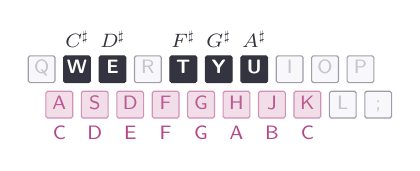
\begin{tikzpicture}
% Upper QWERTY row (sharps in DAW chromatic-staircase). Only 5 keys
% are mapped (W E T Y U); R and I sit in the gaps with no note.
\foreach \l/\note/\mapped [count=\i] in {%
 Q/{}/0, W/$C^\sharp$/1, E/$D^\sharp$/1, R/{}/0, T/$F^\sharp$/1,
 Y/$G^\sharp$/1, U/$A^\sharp$/1, I/{}/0, O/{}/0, P/{}/0%
}{
 \ifnum\mapped=1
  \node[kcap sharp] (k\i) at ({(\i-1)*0.45}, 1.8) {\strut\l};
  \node[font=\scriptsize\sffamily, text=keysharp, anchor=south, inner sep=1pt]
   at ({(\i-1)*0.45}, 2.03) {\note};
 \else
  \node[kcap, text=keystroke!60] (k\i) at ({(\i-1)*0.45}, 1.8) {\strut\l};
 \fi
}
% Home row (whites). 8 of 10 keys mapped (A through K = C..C).
\foreach \l/\note/\mapped [count=\i] in {%
 A/C/1, S/D/1, D/E/1, F/F/1, G/G/1, H/A/1, J/B/1, K/C/1, L/{}/0, {;}/{}/0%
}{
 \ifnum\mapped=1
  \node[kcap mapped] at ({(\i-1)*0.45+0.225}, 1.35) {\strut\l};
  \node[font=\scriptsize\sffamily, text=keymapped, anchor=north, inner sep=1pt]
   at ({(\i-1)*0.45+0.225}, 1.12) {\note};
 \else
  \node[kcap, text=keystroke!60] at ({(\i-1)*0.45+0.225}, 1.35) {\strut\l};
 \fi
}
\end{tikzpicture}}
\caption{Раскладка AWSED --- хроматически-лестничная раскладка QWERTY-фортепиано DAW (вариант Ableton, Logic, GarageBand). Основной ряд \texttt{A~S~D~F~G~H~J~K} играет белые клавиши от $C$ до $C$; ряд выше помещает диезы в зазоры, где легли бы чёрные клавиши фортепиано ($C^\sharp\,D^\sharp$, затем зазор на \texttt{R}, $F^\sharp\,G^\sharp\,A^\sharp$, затем зазоры). Имя происходит от первых пяти хроматических тонов $C\,C^\sharp\,D\,D^\sharp\,E$, которые приходятся на \key{A}\,\key{W}\,\key{S}\,\key{E}\,\key{D}. Буква QWERTY на каждой клавише не имеет отношения к производимому ею имени ноты.}
\label{fig:daw-staircase}
\end{figure}

Она также, как я буду утверждать, плохо спроектирована. У раскладки AWSED три структурные слабости. \textbf{Во-первых}, буква QWERTY на каждой клавише не имеет отношения к производимому ею имени ноты. \key{A} играет C; \key{S} играет D; \key{D} играет E (рисунок~\ref{fig:daw-staircase}). Пользователь, выучивший западную семиступенную гамму, не получает от этого знания никакой опоры в раскладке. \textbf{Во-вторых}, она даёт лишь одну октаву ($C$ до $C$), но растягивает эту одну октаву через весь основной ряд, от \key{A} до \key{K} --- на всю ширину, где покоятся \emph{обе} руки. Это ни компактная одноручная октава, ни продуктивный двуручный диапазон: она тратит клавиатуру на две руки, чтобы произвести единственную октаву, и на том останавливается. Ширина выложена как для двух рук, но диапазон размерен под одну. \textbf{В-третьих}, раскладка нечитаема без учебника: нет мнемоники, нет диаграммы, напечатанной на физических клавишах, и нет способа вывести отображение из первых принципов. Раскладка, требующая руководства, --- это раскладка, утратившая свой социально-программный характер.

Именование было не праздным. Его естественный контраст --- WASD, движенческая конвенция в ПК-играх, --- и почти-анаграмма не столько совпадение, сколько диагноз. WASD имеет ту же структурную форму, что и AWSED, --- никому не принадлежащую, неспецифицированную, межприложенческую конвенцию пользовательского ввода, --- но иную историю распространения. До WASD ПК-игры по умолчанию использовали клавиши-стрелки (Wolfenstein 3D, Doom, серия Quake вплоть до 1997)~\citep{wikipedia_arrow_keys}; промежуточные эксперименты включали ASDX из System Shock (1994) и AZ+QE из Descent. Деннис «Thresh» Фонг, соревновательный игрок в Quake, популяризировал раскладку WASD через своё самиздатское руководство по конфигурации~\citep{thresh_quake_bible} и выиграл первый общенациональный турнир по Quake в 1997 году. Half-Life от Valve поставился с WASD по умолчанию в 1998 году, и к началу 2000-х конвенция насытила ПК-игры~\citep{fenlon2016wasd}. WASD сохраняется по причине, которой нет у хроматической лестницы DAW: она по-настоящему лучше официального умолчания. Она освобождает правую руку для мыши, соседствует с Shift / Space / Ctrl / Tab и эксплуатирует расположение пальцев на основном ряду клавиатуры QWERTY. Структурный урок в том, что распространение есть функция социального опосредования \emph{и} приспособленности: WASD распространилась потому, что педагогика Фонга дошла до игроков, \emph{и} раскладка победила по существу. Хроматическая лестница распространилась через одну педагогику, несмотря на то, что существо было против. Оба случая сидят в одной категории --- никому не принадлежащие конвенции, управляющие пользовательским вводом во множестве приложений. Они показывают, что категория достаточно велика, чтобы охватить и хорошо спроектированное, и плохо спроектированное, и пользовательски проверенное, и унаследованное по инерции.

\section{Notepat.com: ноты, которые сами себя называют}
\label{sec:notepat}

Против этого предшественника \texttt{notepat.com} предлагает иную раскладку (рисунок~\ref{fig:notepat-keymap}). Принцип дизайна единствен: \emph{ноты, которые сами себя называют}. Буква QWERTY \key{C} играет C. Буква QWERTY \key{D} играет D. Семь натуральных нот западной гаммы --- $C\,D\,E\,F\,G\,A\,B$ --- играют ноты, которые называют их буквы. Верхняя октава продолжается по алфавиту: \keys{H,I,J,K,L,M,N} для $C_5\,D_5\,E_5\,F_5\,G_5\,A_5\,B_5$. Диезы располагаются на ряд выше своей натуральной ноты, по аналогии с чёрными клавишами фортепиано, где это позволяют буквы QWERTY: \keys{V,S,W,R,Q} для $C^\sharp\,D^\sharp\,F^\sharp\,G^\sharp\,A^\sharp$. Нижняя октава ложится под левую руку; верхняя --- под правую.

Раскладка обращает каждую из трёх слабостей AWSED. \textbf{Во-первых}, буква на каждой клавише \emph{есть} имя ноты. Всякий, кто знает западную гамму, уже знает раскладку. \textbf{Во-вторых}, она тратит двуручную ширину продуктивно: левая рука играет нижнюю октаву, а правая зеркалит её на верхней, так что тот же размах, что AWSED тратит на одну октаву, даёт две. \textbf{В-третьих}, раскладка самодокументируема: диаграмму на рисунке~\ref{fig:notepat-keymap} может воспроизвести по памяти всякий, кто умеет написать «CDEFGAB».

Три вещи делают \texttt{notepat.com} необычным среди раскладок этой статьи: у него есть имя --- у большинства, как у AWSED (\textsection\ref{sec:daw}), его так и не появилось, --- его ноты сами себя называют, так что раскладка адресует саму себя, и он уже работает во многих реализациях. Вклад \texttt{notepat.com} --- не реализация. Реализация, по замыслу, скромна: несколько сотен строк JavaScript, маршрутизирующих клавиатурные события в API аудиосинтеза. Вклад --- это раскладка. Она представлена в пяти реализациях --- веб-пьесе на \texttt{notepat.com}, голометаллическом порте AC Native OS, приложении строки меню MenuBand для macOS, плагине Ableton (Max for Live) и \texttt{babypat}, --- и раскладка --- та единственная вещь, что идентична во всех них. Нотация именования нот путешествует даже дальше инструмента: она переиспользуется в \texttt{clock}, распределённом секвенсоре AC, где те же однобуквенные высоты управляют сетевым воспроизведением. Это социально-программный договор формы \texttt{notepat.com}.

Читатель, сравнивающий реализации бок о бок, заметит клавиши, делающие вещи сверх таблицы на рисунке~\ref{fig:notepat-keymap}. В AC Native и MenuBand удержание \texttt{Space} воспроизводит в обратном порядке последние несколько секунд фактического аудиовыхода. В веб-пьесе и AC Native удержание \texttt{Shift} при ударе по ноте даёт этому голосу длинный хвост затухания при отпускании; удержание \texttt{Enter} держит голос бесконечно, а \texttt{Backspace} очищает все удерживаемые голоса. В MenuBand и AC Native \texttt{Control}, \texttt{Alt} и оба вместе повышают одно нажатие до мажорного, минорного или уменьшённого трезвучия. Ничего из этого не появляется в диаграмме раскладки, и упущение намеренно. Эти привязки образуют \emph{расширенный исполнительский слой}, и черта между этим слоем и тональным отображением есть граница самого социально-программного договора (таблица~\ref{tab:contract-line}).

\begin{table}[t]
\footnotesize
\setlength{\tabcolsep}{3pt}
\renewcommand{\arraystretch}{1.05}
\centering
\caption{Привязки \texttt{notepat.com}, разделённые по черте договора. Над чертой: тональное отображение, идентичное во всех реализациях, --- социально-программный объект. Под ней: расширенный исполнительский слой, где каждый субстрат волен различаться.}
\label{tab:contract-line}
\begin{adjustbox}{max width=\linewidth,center}%
\begin{tabularx}{\linewidth}{@{}>{\RaggedRight}p{0.30\columnwidth}>{\RaggedRight}X>{\RaggedRight\arraybackslash}p{0.21\columnwidth}@{}}
\toprule
\textbf{Привязка} & \textbf{Значение} & \textbf{Где} \\
\midrule
\multicolumn{3}{@{}l}{\emph{Тональный договор}} \\[0.1em]
\texttt{C D E F G A B} & натуральные $C_4$--$B_4$, левая рука & все \\
\texttt{H I J K L M N} & натуральные $C_5$--$B_5$, правая рука & все \\
\texttt{V S W R Q} & диезы, ряд выше & все \\
\midrule
\multicolumn{3}{@{}l}{\emph{Расширенный исполнительский слой}} \\[0.1em]
\texttt{Shift} (удерж.) & сустейн: длинный хвост затухания & веб, Native \\
\texttt{Enter} (удерж.) & держать голос; \texttt{Backspace} очищает & веб, Native \\
\texttt{Space} (удерж.) & обратное воспроизведение & Native, MenuBand \\
\texttt{Ctrl}\,/\,\texttt{Alt}\,/\,оба & мажор\,/\,минор\,/\,sus2 трезвучие & MenuBand, Native \\
\texttt{<}~\texttt{>} & сдвиг октавы по руке & веб \\
\bottomrule
\end{tabularx}%
\end{adjustbox}
\end{table}

Две половины таблицы~\ref{tab:contract-line} управляются разными правилами. Над чертой отклонение есть поломка: реализация, переотобразившая \texttt{C} прочь от ноты $C$, была бы не портом \texttt{notepat.com}, а иным инструментом. Под чертой отклонение есть идиома: каждый субстрат отращивает жесты, которые позволяет его тело. Голометаллическая ОС, владея всей машиной, может кольцевать собственный аудиовыход и проигрывать его задом наперёд; приложение строки меню, оседлав общесистемный перехват событий, опирается на аккорды модификаторов; веб-пьеса, живущая во вкладке браузера, сустейнит и держит. Пользователи не переживают эти различия как поломку, и ни одна реализация не обязана нести жесты другой. Та же двухъярусная структура видна в более старых случаях: QWERTY-как-договор ничего не говорит о медиаклавишах или слоях \texttt{Fn}, которые свободно варьируются от производителя к производителю, и никто не зовёт ThinkPad форком QWERTY; ядровые движения Vim суть договор, а привязки плагинов --- идиома. Раскладка, подсказывает это, --- не набор всех привязок, которые поставляет реализация. Это подмножество, чьё изменение сообщество пережило бы как нарушение идентичности, --- и один практический тест на то, по какую сторону черты падает привязка, --- несёт ли её поверхность нотации (\textsection\ref{sec:notation}). \texttt{C D E F G A B} путешествует как текст; «удержи space, чтобы обратить время» --- жест на каждый субстрат, который надо переучивать, по показу, при каждом порте.

Это и есть тот ход, который статья просит читателя увидеть. Доминирующая хроматически-лестничная раскладка DAW никогда не была \emph{выбрана} --- она была \emph{унаследована} от трекерного ПО, удержана пользовательским ожиданием и заблокирована межприложенческой конвенцией. \texttt{notepat.com} показывает, что лакуна открыта: что намеренно спроектированную альтернативу может написать один разработчик в несколько сотен строк кода, поставить в нескольких реализациях за год и предложить более широкому сообществу как конкурирующий социально-программный договор. Политическая ставка мала в любом отдельном случае и велика в совокупности: \emph{лакуна открыта повсюду}.

\section{Нотация: дискурсивная поверхность}
\label{sec:notation}

Аргумент до сих пор трактовал раскладку как таблицу. Но раскладка --- не только таблица. У неё есть ещё и \emph{нотация} --- текстовая форма, в которой употребление раскладки читается, пишется, преподаётся, цитируется и оспаривается. Нотация --- дискурсивная поверхность раскладки. Это также, как я буду утверждать, та половина раскладки, что действительно путешествует. Раскладка, чья нотация переносима, распространяется как текст; раскладка, чья нотация неуклюжа или отсутствует, распространяется лишь как мышечная память. Качество нотации --- поэтому проектируемое свойство раскладки, а не производный артефакт. Дизайнер, поставивший лишь таблицу привязок, поставил половину объекта.

Канонический случай --- Vim. Лежащая в основе раскладка Vim --- таблица, сопоставляющая нажатия командам редактора: \texttt{d} инициирует оператор удаления, \texttt{i} --- внутренний текстовый объект, \texttt{w} --- движение по слову. То, что путешествует в дискурсе Vim, однако, --- не таблица. Путешествует \emph{нотация}: \texttt{dd}, \texttt{ciw}, \texttt{gg}, \texttt{:wq}, \texttt{<C-w>} (рисунок~\ref{fig:vim-modes}). Учебники, посты в блогах, файлы README, vimtutor и долгоиграющий спор vim-против-emacs --- все ведутся в этой нотации. Нотация столь переносима, что выживает вовсе вне Vim: \emph{vim-режим} появляется в Visual Studio Code, в JupyterLab, в оболочках через \texttt{set -o vi}, в текстовых полях macOS Cocoa, в браузерах через Vimium. То, что портируется, --- нотация. Среда исполнения случайна.

\begin{figure}[t]
\centering
\begin{tikzpicture}[
 modebox/.style={draw=keymapped!70, fill=keymapped!12,
          rounded corners=2pt, minimum width=1.6cm,
          minimum height=0.6cm, font=\small\sffamily,
          text=keymapped!90, inner sep=2pt},
 arrow/.style={-{Stealth[length=4pt,width=4pt]}, draw=keystroke!90,
         line width=0.5pt},
 cmd/.style={font=\footnotesize\ttfamily, text=acdark}
]
% Three Vim modes wired by their command-notation transitions.
\node[modebox] (normal) at (0, 0) {NORMAL};
\node[modebox] (insert) at (3.0, 0) {INSERT};
\node[modebox] (visual) at (-3.0, 0) {VISUAL};
\draw[arrow] ([yshift=4pt]normal.east) -- node[above, cmd] {\texttt{i}\,/\,\texttt{a}\,/\,\texttt{o}} ([yshift=4pt]insert.west);
\draw[arrow] ([yshift=-4pt]insert.west) -- node[below, cmd] {\texttt{<Esc>}} ([yshift=-4pt]normal.east);
\draw[arrow] ([yshift=4pt]normal.west) -- node[above, cmd] {\texttt{v}\,/\,\texttt{V}\,/\,\texttt{<C-v>}} ([yshift=4pt]visual.east);
\draw[arrow] ([yshift=-4pt]visual.east) -- node[below, cmd] {\texttt{<Esc>}} ([yshift=-4pt]normal.west);
% A row of canonical commands underneath
\node[font=\footnotesize\ttfamily, text=acdark, anchor=north] at (0, -1.0)
 {\texttt{dd}\,\,\texttt{ciw}\,\,\texttt{gg}\,\,\texttt{:wq}\,\,\texttt{<C-w>v}\,\,\texttt{y2}\$};
\end{tikzpicture}
\caption{Модальная раскладка Vim и её путешествующая нотация. Режимы (NORMAL, INSERT, VISUAL) соединены помеченными переходами по нажатиям; распространённые команды (\texttt{dd} удалить строку, \texttt{ciw} изменить внутреннее слово, \texttt{gg} к началу, \texttt{:wq} записать и выйти и т.д.) --- дискурсивная валюта раскладки. Нотация столь переносима, что перереализована в VS~Code, JupyterLab, Vimium, текстовой системе macOS Cocoa и \texttt{set -o vi}.}
\label{fig:vim-modes}
\end{figure}

Хроматическая лестница DAW --- отрицательный случай. Для неё нет переносимой нотации. Запись мелодии, сыгранной на музыкальной печати Ableton, требует отката к прозе последовательности событий --- «нажмите \key{A}, затем \key{S}, затем \key{D}» --- которая описывает ввод, а не музыку. Сравните с кубической нотацией Сингмастера~\citep{singmaster1981notes} (рисунок~\ref{fig:singmaster}), где \texttt{R U R' U' R U2 R'} позволяет алгоритму кубика Рубика путешествовать невредимым между куберами; или с Нэшвиллской числовой системой~\citep{matthews1984nashville,williams1988nashville}, где «1--4--5» позволяет аккордовой прогрессии путешествовать между сессионными музыкантами; или со стенотеорией Plover~\citep{knight2010plover}, где аккордовая нотация позволяет стенографическим паттернам путешествовать через словарь, редактируемый сообществом. У DAW-лестницы нет такой ручки. Её клавиши адресуемы лишь по физической позиции. Раскладка поэтому существует в мышечной памяти и редко на странице --- именно поэтому у неё ниже дискурсивное присутствие, чем у Vim, несмотря на, пожалуй, бóльшую пользовательскую базу.

\begin{figure}[t]
\centering
\resizebox{0.62\columnwidth}{!}{%
\begin{tikzpicture}
% Symmetric bounding box around the cube body (x=0) so \centering
% lands it centered --- the quarter-turn arrow otherwise extends the
% natural box rightward and pulls the cube off-center.
\useasboundingbox (-1.85,-2.55) rectangle (1.85,1.55);
% Isometric Rubik's cube, three visible faces: U (top), F (front-
% left), R (right). Faces are explicit-path parallelogram grids built
% from iso axes er=(0.866,0.5)s (right-up), el=(-0.866,0.5)s
% (left-up), ed=(0,-1)s (down), all meeting at the shared front-top
% vertex at the origin. The R face is tinted with a quarter-turn
% arrow: the diagram shows the first move of the algorithm below.
\def\s{0.55}
% Top face U: cells spanned by er and el
\foreach \i in {0,1,2} \foreach \j in {0,1,2}
 \draw[keystroke, fill=keyfill]
  ({0.866*\s*(\i-\j)}, {0.5*\s*(\i+\j)})
  -- ++({0.866*\s}, {0.5*\s})
  -- ++({-0.866*\s}, {0.5*\s})
  -- ++({-0.866*\s}, {-0.5*\s}) -- cycle;
% Front-left face F: cells spanned by el and ed — green stickers
\foreach \i in {0,1,2} \foreach \j in {0,1,2}
 \draw[acgreen!75!black, fill=acgreen!55]
  ({-0.866*\s*\i}, {0.5*\s*\i - \s*\j})
  -- ++({-0.866*\s}, {0.5*\s})
  -- ++(0, {-\s})
  -- ++({0.866*\s}, {-0.5*\s}) -- cycle;
% Right face R: cells spanned by er and ed — red stickers (mid-turn)
\foreach \i in {0,1,2} \foreach \j in {0,1,2}
 \draw[red!70!black, fill=red!55]
  ({0.866*\s*\i}, {0.5*\s*\i - \s*\j})
  -- ++({0.866*\s}, {0.5*\s})
  -- ++(0, {-\s})
  -- ++({-0.866*\s}, {-0.5*\s}) -- cycle;
% Face labels at face centers — standard sticker scheme:
% white up, green front, red right.
\node[font=\small\sffamily\bfseries, text=acdark]
 at (0, {1.5*\s + 0.5*\s}) {U};
\node[font=\small\sffamily\bfseries, text=white]
 at ({-0.866*\s*1.5 - 0.433*\s}, {0.75*\s - 1.5*\s + 0.25*\s}) {F};
\node[font=\small\sffamily\bfseries, text=white]
 at ({0.866*\s*1.5 + 0.433*\s}, {0.75*\s - 1.5*\s + 0.25*\s}) {R};
% Quarter-turn arrow for R: curved arrow hugging the right face's
% outer edge, pointing upward (clockwise as seen from the right).
\draw[-{Stealth[length=5pt,width=5pt]}, line width=1.1pt, red!70!black]
 ({0.866*\s*3.45}, {0.5*\s*3.45 - 2.5*\s})
 to[bend right=42]
 ({0.866*\s*3.45}, {0.5*\s*3.45 - 0.35*\s});
% Notation row underneath
\node[font=\small\ttfamily, anchor=north, text=acdark]
 at (0, {-3.2*\s}) {R\,U\,R$'$\,U$'$\,R\,U2\,R$'$};
\node[font=\scriptsize\sffamily, anchor=north, text=keystroke]
 at (0, {-4.0*\s}) {алгоритм из 7 ходов};
\end{tikzpicture}}
\caption{Кубическая нотация Сингмастера~\citep{singmaster1981notes}. Каждая заглавная буква именует грань (\textsf{U}p --- верх, \textsf{D}own --- низ, \textsf{L}eft --- лево, \textsf{R}ight --- право, \textsf{F}ront --- перёд, \textsf{B}ack --- зад); голая буква --- поворот на четверть по часовой стрелке, штрихованная буква ($\,'$) --- против часовой, а цифра-2 --- полуоборот. Строка из семи токенов \texttt{R U R$'$ U$'$ R U2 R$'$} --- полный алгоритм, переносимый между куберами, репозиториями GitHub и видеоуроками YouTube, --- пара раскладка-нотация, путешествующая как текст. Грани несут стандартную схему наклеек (белый --- верх, зелёный --- перёд, красный --- право); \textsf{R} нарисована в середине четвертьповорота: первый ход алгоритма.}
\label{fig:singmaster}
\end{figure}

У дизайна «ноты-себя-называют» от \texttt{notepat.com} есть, как структурный побочный эффект, нотация, выучивание которой ничего не стоит. Чтобы записать последовательность notepat.com, пишут \texttt{C D E F G A B} --- что есть также стандартная музыкальная нотация. Нотация не изобретена для \texttt{notepat.com}; она \emph{унаследована} от существующей грамотности. Пианист, никогда не видевший раскладки notepat.com, может прочитать партитуру notepat.com; и наоборот, исполнитель notepat.com, выучивающий раскладку, заодно репетирует стандартную буквенно-высотную грамотность. Вот как выглядит хорошо спроектированная поверхность нотации: нотация столь тривиально выводима из предшествующего знания, что её выучивание ничего не стоит. Хроматическая лестница Ableton, напротив, потребовала бы перекодировать notepat-подобную партитуру как \texttt{A S D F G H J} --- приватную нотацию, привязанную к одной раскладке, бесполезную больше нигде.

Эмпирическая литература о принятии клавиатурных сочетаний поддерживает это прочтение. Перес и др.\ обнаружили, что работа бок о бок с другими пользователями сочетаний --- более сильный предиктор использования сочетаний, чем один лишь компьютерный опыт~\citep{peres2004shortcut}. Ложкина и др.\ расширяют результат: канал открытия сочетаний межличностный и визуальный~\citep{lozhkina2025discovery}. Ван и др.\ явно используют термин \emph{словарь}, чтобы назвать то, что дизайн сочетаний вручает пользователю~\citep{wang2020keymap}. Аргумент этой статьи заостряет эти находки: социальное опосредование --- не родовой эффект пребывания-среди-других-пользователей; это конкретная передача через поверхность нотации. Коллеги читают экраны друг друга, видят \texttt{:wq}, спрашивают, учатся. Где нет передаваемой нотации, там нет и социального опосредования, чтобы опосредовать. Та же логика объясняет успех мини-нотаций живого кодинга: язык паттернов TidalCycles Алекса Маклина и Герайнта Уиггинса~\citep{mclean2010tidal}, портированный в JavaScript как Strudel~\citep{roos2023strudel}, и цепочки преобразований Hydra Оливии Джек для живокодируемой визуалистики~\citep{jack2018hydra}, наряду с нотацией ABC для фолк-музыки~\citep{walshaw_abc}. В каждом случае среда исполнения случайна --- Haskell, JavaScript, WebGL, MIDI-плееры, --- но нотация несёт практику сквозь среды, мастерские и десятилетия.

Каталог следствий из \textsection\ref{sec:corollaries}, прочитанный сквозь эту линзу, почти целиком есть каталог нотаций. Сингмастер, Нэшвилл, ABC, IPA, Camelot, нумпад-нотация файтингов, научная высота звука, фонетический алфавит НАТО, вязальные сокращения --- каждое есть нотация, выведенная из раскладки (или отображения ввода), которая позволила лежащей в основе практике путешествовать как текст. Пара раскладка-нотация --- единица. Раскладка даёт аффорданс; нотация даёт поверхность распространения.

Структурное утверждение имеет более глубокий диагностический смысл. Различение Уолтера Онга между устностью и письменностью~\citep{ong1982orality}, опирающееся на изложение Хэвлоком того же перехода в Древней Греции~\citep{havelock1963preface}, рассекает вопрос начисто. \emph{Устные} традиции сохраняются через исполнение, передачу от человека к человеку и повторное приближение; у них нет канонического текста, они слегка мутируют от случая к случаю и выживают потому, что исполнители продолжают их исполнять. \emph{Письменные} традиции сохраняются через фиксированный текст, авторитетные издания и точное воспроизведение; у них есть спецификации, каноны и эталонные реализации. Стандартные рамки академических исследований вычислений все суть письменные рамки: открытая лицензия управляет фиксированным текстом, протокол управляет фиксированным сетевым форматом, формат управляет фиксированным кодированием. Хроматическая лестница DAW --- первично-устная раскладка: нет канонического текста, лишь четыре реализации, согласные по исполнению. У Vim есть и устный субстрат (раскладку учат, глядя на экран другого разработчика), и письменный край (нотация: \texttt{:wq}, \texttt{<C-w>}, \texttt{ciw}). \texttt{notepat.com} сворачивает письменную сторону в стоящую грамотность буквенно-высотной нотации: раскладка наследует свою письменную форму от практики на столетия старше. Устный субстрат --- раскладка; нотация --- письменная фиксация; где последняя удаётся, первая обретает тело, которое путешествует. Ось устности-письменности --- диагноз того, почему раскладки вообще ускользают от рамки «открытый код/проприетарный»: стандартные рамки суть письменные рамки, но раскладка по меньшей мере отчасти устна, и отсутствие письменной фиксации как в академическом, так и в индустриальном дискурсе --- симптом, давший этой статье её мотивирующий вопрос.

Та же ось устности-письменности объясняет особенность литературы о раскладках: её немного. История WASD от PC Gamer~\citep{fenlon2016wasd} --- канонический популярно-публицистический источник о конвенции, управляющей сотнями миллионов часов геймплея; эквивалентная академическая литература по сути пуста. Это не потому, что раскладки неважны. Это потому, что существующий аппарат академических исследований вычислений --- спецификации, RFC, репозитории исходного кода --- откалиброван под письменные артефакты, а раскладка отчасти устна. Статья, которой не существует, --- ровно та, которая, как утверждает эта статья, должна существовать.

\section{Каталог следствий}
\label{sec:corollaries}

Раскладка --- один экземпляр гораздо большего рода: \emph{версионируемых виртуальных объектов, распространяющихся через общественный договор, а не через бинарники}. Таблица~\ref{tab:corollaries} каталогизирует основные виды. Каталог не исчерпывающ. Его цель --- показать, что род реален и велик.


Проступает несколько паттернов. Во-первых, род охватывает отображения ввода (QWERTY, Vim, WASD), нотационные системы (Сингмастер, Нэшвилл, IPA), категориальные ярлыки (кнопки контроллера, именованные цвета CSS) и созданные сообществом инициализмы (фонетический алфавит НАТО; акроним LGBTQ+, чья история ревизий --- LGB $\rightarrow$ LGBT $\rightarrow$ LGBTQ $\rightarrow$ LGBTQIA $\rightarrow$ LGBTQIA2S+ --- сама есть процесс версионирования-без-управляющего-органа, задокументированный в руководствах по стилю~\citep{glaad_reference_guide}). Объединяет их не среда, а \emph{роль}: каждое есть небольшая декларативная таблица, к которой обращаются на границе между человеком и машиной, между сообществами практики или между конкурирующими реализациями. Во-вторых, паттерн именованного-изобретателя крайне изменчив. У одних объектов есть единственный именованный изобретатель (Сингмастер, Coleman, Davis); у других --- конвергентные или анонимные истоки (хроматическая лестница DAW, нумпад-нотация файтингов); третьи версионируются сообществом с именованными добавлениями (инициализм LGBTQ+); четвёртые кристаллизованы федерацией после периода конкуренции сообществ (алгебраические шахматы, BÉPO). В-третьих, механизм распространения почти всегда \emph{не} бинарник. Это педагогика, ожидание, цитирование или письменная отсылка --- аппарат письменного сообщества.

Границу категории стоит провести чётко. \textbf{Открытые форматы} вроде PNG и MP3 управляются спецификациями и эталонными реализациями~\citep{sterne2012mp3} --- ближе к формату, чем к социальному ПО. \textbf{Открытые протоколы} вроде HTTP и IRC имеют RFC и распорядительные органы --- \emph{Protocol} Галлоуэя~\citep{galloway2004protocol} покрывает эту территорию. \textbf{Фолксономии} (теги, хэштеги) суть классификация контента, а не интерфейс-как-объект. \textbf{Мемы} распространяются, но суть контент. Раскладка отлична от всех них: \emph{небольшая декларативная таблица, опосредующая ввод/вывод, без управляющего органа, которая тем не менее ведёт себя как стандартизированная}.

% X cells render as m{} (vertically centered, footnotesize) so single
% -line labels sit centered against wrapped propagation text. Defined
% OUT here (not inside \afterpage — a bare #1 breaks its tokenizer).
\renewcommand{\tabularxcolumn}[1]{>{\footnotesize}m{#1}}
% Full-width table as a proper float page ([p]): LaTeX fills the
% surrounding two-column text pages completely (no stranded column)
% and drops the table on its own float page. Label columns auto-size
% and never wrap; only the Propagation column flexes.
\begin{table*}[p]
\footnotesize
\setlength{\tabcolsep}{5pt}
\renewcommand{\arraystretch}{1.32}
\centering
\caption{Избранные версионируемые виртуальные объекты, распространяющиеся через общественный договор. «Создатель» приводит именованного изобретателя там, где он есть; «\emph{конв.}» указывает на конвергентный или анонимный исток. QR-код каждого ряда ведёт к каноническому дому объекта --- Wikipedia, собственному сайту проекта или его управляющей спецификации.}
\label{tab:corollaries}
\arrayrulecolor{acgray!35}
\begin{adjustbox}{max width=\linewidth,center}%
\begin{tabularx}{\linewidth}{|@{\hspace{2.5pt}}c@{\hspace{2.5pt}}|>{\bfseries\color{acdark}}l|>{\color{acdark}}l|l|>{\RaggedRight\arraybackslash\color{acdark}}X|}
\hline
\cellcolor{acdark!75}{\color{white}\bfseries Скан} &
\cellcolor{acpink!75}{\color{white}\bfseries Объект} &
\cellcolor{acpurple!75}{\color{white}\bfseries Создатель (год)} &
\cellcolor{acblue!75}{\color{white}\bfseries Область} &
\cellcolor{acgreen!75}{\color{white}\bfseries Распространение} \\
\hline
\rowcolor{acblue!8} \qrc{qwerty} & QWERTY            & Sholes (1873)               & \dmn{acblue}{Печать}  & Принятие производителями $\rightarrow$ ISO/AFNOR $\rightarrow$ файлы раскладок ОС \\ \hline
\rowcolor{acblue!8} \qrc{dvorak} & Dvorak            & Dvorak \& Dealey (1936)          & \dmn{acblue}{Печать}  & Патент США $\rightarrow$ ВМС США $\rightarrow$ раскладки ОС, ставимые пользователем \\ \hline
\rowcolor{acblue!8} \qrc{colemak} & Colemak           & Coleman (2006)               & \dmn{acblue}{Печать}  & colemak.com + форки GitHub (Workman, Halmak, DH) \\ \hline
\rowcolor{acblue!8} \qrc{bepo} & BÉPO             & Community (2005)              & \dmn{acblue}{Печать}  & Дизайн сообщества $\rightarrow$ гос. стандарт AFNOR 2019 \\ \hline
\rowcolor{acpink!8} \qrc{janko} & Janko            & Jankó (1882)                & \dmn{acpink}{Музыка}   & \emph{Провал распространения} --- отрицательный кейс \\ \hline
\rowcolor{acpink!8} \qrc{wicki} & Wicki--Hayden         & Wicki (1896) / Hayden (1986)        & \dmn{acpink}{Музыка}   & Сообщество концертины $\rightarrow$ современные MPE-контроллеры \\ \hline
\rowcolor{acpink!8} \qrc{bosanquet} & Bosanquet          & Bosanquet (1875)              & \dmn{acpink}{Музыка}   & Микротональное сообщество $\rightarrow$ Lumatone \\ \hline
\rowcolor{acpink!8} \qrc{daw} & AWSED (лестница DAW) & \emph{конв.} (трекеры, 1990-е)       & \dmn{acpink}{Музыка}   & МежDAW-педагогика; пользовательское ожидание \\ \hline
\rowcolor{acgreen!8} \qrc{wasd} & Движение WASD        & Fong (1996--97)              & \dmn{acgreen}{Игры}  & Педагогика Quake $\rightarrow$ умолчание Half-Life $\rightarrow$ норма индустрии~\citep{fenlon2016wasd,thresh_quake_bible} \\ \hline
\rowcolor{acpink!8} \qrc{notepat} & Notepat «сами называются» & Scudder (2024)               & \dmn{acpink}{Музыка}   & Межреализационный договор внутри \ac{} \\ \hline
\rowcolor{acblue!8} \qrc{plover} & Стенотеория Plover     & Knight (2010-е)               & \dmn{acblue}{Печать}  & GitHub + форкнутые сообществом словари \\ \hline
\rowcolor{acpurple!8} \qrc{vim} & Привязки Vim       & Joy (1976) $\rightarrow$ Moolenaar (1991) & \dmn{acpurple}{Редактирование} & «Привязки Vim повсюду»; текстовые поля macOS Cocoa \\ \hline
\rowcolor{acorange!8} \qrc{singmaster} & Нотация Сингмастера     & Singmaster (1981)             & \dmn{acorange}{Головоломка} & Брошюра Penguin $\rightarrow$ всеобщее принятие куберами \\ \hline
\rowcolor{acorange!8} \qrc{chess} & Алгебраическая шахматная нотация   & Stamma (1737) $\rightarrow$ FIDE (1981)  & \dmn{acorange}{Игра}  & Федеративная кристаллизация конвенций сообщества \\ \hline
\rowcolor{acpink!8} \qrc{nashville} & Нэшвиллская числовая система   & Matthews (1957) / Williams (1988)     & \dmn{acpink}{Музыка}   & Устная традиция сессионных музыкантов + самиздат \\ \hline
\rowcolor{acpink!8} \qrc{abc} & Нотация ABC         & Walshaw (1980-е)              & \dmn{acpink}{Музыка}   & Текстовый обмен фолк-мелодиями в рассылках \\ \hline
\rowcolor{acpink!8} \qrc{helmholtz} & Гельмгольц / научная высота & Helmholtz (1863) / Sauveur (1713)     & \dmn{acpink}{Музыка}   & Учебники акустики + документация MIDI \\ \hline
\rowcolor{acpink!8} \qrc{camelot} & Колесо Camelot        & Davis (1991)                & \dmn{acpink}{Диджеинг}   & Mixed In Key + всякий инструмент определения тональности \\ \hline
\rowcolor{acgreen!8} \qrc{numpad} & Нумпад-нотация (236P)    & \emph{конв.} (япон. FGC)        & \dmn{acgreen}{Игры}  & Вики, сабреддиты подбора игр \\ \hline
\rowcolor{acpink!8} \qrc{tidal} & Мини-нотация TidalCycles  & McLean \& Wiggins (2010)          & \dmn{acpink}{Музыка}   & Tidal Club + мастерские + паттерны GitHub~\citep{mclean2010tidal} \\ \hline
\rowcolor{acpink!8} \qrc{strudel} & Мини-нотация Strudel    & Roos \& McLean (2023)           & \dmn{acpink}{Музыка}   & Браузерный редактор + педагогика ICLC~\citep{roos2023strudel} \\ \hline
\rowcolor{acpink!8} \qrc{hydra} & Цепочки преобразований Hydra    & Jack (2018)                & \dmn{acpink}{Визуалистика}  & Браузер + общие гисты~\citep{jack2018hydra} \\ \hline
\rowcolor{acgray!12} \qrc{ipa} & IPA             & IPA Association (1888)           & \dmn{acgray}{Фонетика} & Стандартизирована федерацией; пересмотрена в Киле 1989 \\ \hline
\rowcolor{acgray!12} \qrc{nato} & Фонетический алфавит НАТО    & ICAO (1956)                & \dmn{acgray}{Авиация} & Стандартизирован федерацией \\ \hline
\rowcolor{acgray!12} \qrc{lgbtq} & Инициализм LGBTQ+      & Community (1980-е--)            & \dmn{acgray}{Идентичность} & Руководства по стилю (GLAAD); пересмотрен через употребление~\citep{glaad_reference_guide} \\ \hline
\rowcolor{acgreen!8} \qrc{controller} & Кнопки контроллера      & Nintendo (1990) / Goto (1994)       & \dmn{acgreen}{Игры}  & Порты несут оба набора ярлыков (A/B/X/Y \emph{против}\ $\triangle\,\bigcirc\,\times\,\mdlgwhtsquare$) \\ \hline
\rowcolor{acgray!12} \qrc{css} & Именованные цвета CSS       & X11 (1987) $\rightarrow$ SVG (2001)    & \dmn{acgray}{Веб}    & Унаследованы неизменными во всех браузерах \\ \hline
\rowcolor{acgray!12} \qrc{knitting} & Вязальные сокращения    & Craft Yarn Council / UK          & \dmn{acgray}{Ремесло}   & Печатаются в каждом паттерне \\ \hline
\end{tabularx}%
\end{adjustbox}
\arrayrulecolor{black}
\end{table*}

\section{Чтение сквозь Лиалину}
\label{sec:lialina}

Эссе Оли Лиалиной \emph{Turing Complete User}~\citep{lialina2012turing,lialina2021turingbook} --- несущий теоретический якорь этой статьи. Лиалина утверждает, что категория «пользователь» тихо устраняется из современного дизайна ПО, заменяясь регистром, который обращается к людям, не признавая той деятельности, что сделала их пользователями в первую очередь. Аргумент моральный и политический: «Нам нужно заботиться об этом слове, потому что обращение к людям, а не к пользователям, скрывает существование двух классов людей --- разработчиков и пользователей»~\citep{lialina2012turing}. Её тезис в том, что пользователи суть программисты в ожидании; субстрат должен оставаться программируемым, чтобы деятельность была реальной.

Раскладка, утверждаю я, --- ровно та поверхность, где аргумент Лиалиной находит материальное выражение. Лиалина именует условие, делающее пользовательское авторство возможным: «ситуация, когда рабочий поток приложения имеет лакуны, которые могут быть заполнены пользователями, где гладкость и бесшовность нарушены»~\citep{lialina2012turing}. Раскладка --- такая лакуна. Аппаратура фиксирована; бинарник закрыт; но таблица, сопоставляющая клавишу QWERTY \key{A} с MIDI 60, авторизуема пользователем, версионируема пользователем и востребована пользователем во множестве приложений. Когда приложения закрывают эту лакуну --- вшивают одно отображение, отвергают альтернативы, прячут таблицу за слоем UX, не допускающим правок, --- пользователь-как-автор умирает на этой поверхности. Это то, что Лиалина в своём сопутствующем эссе~\citep{lialina2018rich} называет \emph{десктопизацией}: колонизацией пользовательски конфигурируемых поверхностей управляемым UX. Раскладка --- канарейка.

Каталог следствий из \textsection\ref{sec:corollaries} заостряет мысль. Каждая запись в таблице~\ref{tab:corollaries} --- поверхность, на которой пользовательское сообщество авторски создало небольшую декларативную таблицу, которую лежащая в основе технология не требовала. Западная гамма не требует нотации ABC; клавиатура QWERTY не требует стенотеории Plover; кубик Рубика не требует нотации Сингмастера; хроматическая 12-тоновая равномерно-темперированная гамма не требует раскладки «сами-называются» от notepat.com. Каждая --- кусок пользовательски-авторской конвенции, что выживает и распространяется потому, что сообщество решило, что так должно быть.

Политическая ставка \emph{Turing Complete User} --- сохранение этих поверхностей. Вклад этой статьи --- дать поверхностям имя --- \emph{социальное ПО} --- и продемонстрировать, через перечисление, что категория достаточно велика, чтобы быть политически значимой. Аргумент \textsection\ref{sec:notation} заостряет политическое притязание: где у раскладки есть переносимая нотация, авторство пользователя читаемо для других пользователей; где её нет, раскладка умирает в мышечной памяти, и социально-программный договор становится невидимым даже для тех, кто его держит. Исчезновение какой-либо одной раскладки мало. Исчезновение всего пользовательски-авторского слоя --- это исчезновение пользователя Лиалиной. Исчезновение \emph{поверхности нотации} --- это исчезновение голоса пользователя в дополнение к руке пользователя.

\section{Чего это требует от дизайнеров}
\label{sec:design}

Если аргумент \textsection\ref{sec:lialina} верен --- если раскладки суть эмпирическое тело Тьюринг-полного пользователя, --- то для дизайнеров любой системы, потребляющей раскладку, следует небольшая конкретная просьба. \textbf{Поставляйте раскладку как полноправный объект.} Сделайте её читаемой: напечатайте таблицу где-нибудь, где пользователь может её увидеть. Сделайте её экспортируемой: позвольте пользователю сохранить таблицу в файл. Сделайте её форкаемой: позвольте пользователю загрузить иную таблицу. Сделайте формат задокументированным: предпочитайте обычную текстовую таблицу непрозрачному бинарнику. Предпочитайте опубликованную конвенцию приватной. Предпочитайте раскладку, разделяемую сообществом, той, что принадлежит лишь вендору.

\textbf{И поставляйте нотацию как полноправный объект тоже} (\textsection\ref{sec:notation}). Раскладка --- половина артефакта; нотация --- другая половина. Раскладка, чья нотация неуклюжа, нетранскрибируема или изобретена с нуля, будет дремать в мышечной памяти. Раскладка, чья нотация лаконична, типографична и выводима из существующей грамотности сообщества, будет путешествовать как текст, распространяться через учебники и пережить свою нынешнюю среду исполнения. Два вопроса дизайна неразделимы: выбирая привязку, вы выбираете заодно, как об этой привязке будут писать, как ей учить и как её портировать.

\texttt{notepat.com} поставляет свою раскладку как рисунок~\ref{fig:notepat-keymap} --- одностраничную диаграмму, свободно воспроизводимую, присутствующую в каждой реализации. Хроматическая лестница DAW поставляет свою раскладку как учебник, погребённый в руководстве, идентичный во всех приложениях по случайности, не принадлежащий никому и неоспоримый никем. Различие не техническое. Различие в том, трактуется ли социально-программный договор как явный объект или как неявный.

\section{Заключение}

Раскладка --- небольшая декларативная таблица. Это не бинарник. Это не сервис. Это не проект. Стандартные рамки академических исследований вычислений её не различают. И тем не менее раскладки версионируемы, именуемы, форкаемы и востребованы во множестве приложений --- они суть ПО во всяком смысле, который имеет значение. Я утверждал, что они образуют категорию, назвал эту категорию \emph{социальным ПО}, проследил две породившие её линии, рассмотрел доминирующий современный случай (хроматическую лестницу DAW) и намеренное вмешательство против него (ноты-которые-сами-называются от \texttt{notepat.com}), показал, что у каждой раскладки есть \emph{поверхность нотации}, которая часто и есть та половина артефакта, что действительно путешествует, перечислил более широкий каталог следствий, которые сами по преимуществу суть нотации, и прочитал корпус свидетельств сквозь \emph{Turing Complete User} Лиалиной как поддержку её тезиса о том, что пользователи суть программисты в ожидании. Исчезновение какой-либо одной раскладки мало. Исчезновение всего пользовательски-авторского слоя --- это политическая проблема, которую именует Лиалина.

Методологический вклад --- единица анализа: раскладка-и-её-нотация как полноправный объект академических исследований вычислений, который бинарник, проект, платформа и формат вместе не могут разрешить. Прочитанная сквозь Онга, раскладка --- отчасти-устный артефакт, а нотация --- её письменный край, --- вот почему ни раскладка одна, ни нотация одна не достаточны, и почему стандартные рамки академических исследований вычислений, откалиброванные, как они есть, под полностью-письменные артефакты, целиком упускают категорию. Политический вклад --- небольшая просьба: \emph{поставляйте раскладку как полноправный объект и нотацию вместе с ней}.

\section*{Благодарности}

Эта статья написана во время резиденции автора в \emph{Social Software}, инициативе в UCLA Design\,\textbar\,Media Arts под руководством Lauren Lee McCarthy и Casey Reas~\citep{sosoft_info}, в рамках её второго цикла, \emph{Scores for Social Software}, под руководством Casey Reas, апрель--июнь 2026~\citep{reas2026scores}. Рамка цикла, прочитывающая партитуру как способ хореографии событий во времени посредством текста, диаграмм и иных форм инструкции, сформировала аргумент о нотации в \textsection\ref{sec:notation}, а определение социального ПО, данное инициативой, --- любая система, организующая поведение, координирующая людей или структурирующая взаимодействие, --- есть рабочий контекст для категории, которую именует эта статья. Спасибо когорте за десять недель партитур.\hspace{3pt}\raisebox{-5pt}{\rotatebox{-12}{
\includegraphics[height=26pt]{figures/pals-pink.png}}}

\appendix
\renewcommand{\thesection}{Приложение~\Alph{section}}

\section{Раскладка и модуль: Notepat после Джона Холдена}
\label{app:holden}

В 1770 году глазговский гончар по имени Джон Холден опубликовал \emph{Essay towards a Rational System of Music}, который, как показала Кармел Раз, предвосхитил когнитивную науку на два столетия~\citep{holden1770,raz2025}. Работая с псалмовыми напевами и народными мелодиями --- его «нянюшкиными напевами», --- Холден утверждал, что слышание музыки есть акт \emph{памяти}: ум выводит интернализированный эталон из ключевой ноты и держит его как опору, относительно которой всякая последующая высота группируется и сравнивается. Он назвал этот запомненный эталон \emph{модулем} --- не вещью в воздухе или на странице, а конструктом, который слушатель поддерживает, так что «ранее удержанные модули\ldots в имплицитной памяти прямо влияют на восприятие новых звуков»~\citep{raz2025}. Сопутствующая статья прослеживает, как \ac{} сходится к этой программе на уровне среды исполнения~\citep{scudder2026holden}; здесь же я хочу мельчайшую версию утверждения, на уровне раскладки.

Раскладка, прочитанная сквозь Холдена, --- модуль, вывернутый наизнанку. Там, где его модуль --- запомненный каркас, который строит единственный слушатель, чтобы разбирать входящий звук, раскладка --- запомненный каркас, который \emph{сообщество} соглашается разделять, --- тот же род эталона, экстернализованный и сделанный социальным. Вот почему дизайн таблицы есть дизайн о памяти. Раскладка AWSED (\textsection\ref{sec:daw}) требует нового модуля: ничто из того, что игрок уже знает, не переносится, так что отображение должно ставиться зубрёжкой и держаться усилием, и в миг, когда внимание ослабевает, раскладка растворяется. \texttt{notepat.com} делает противоположную ставку. Позволяя букве \key{C} играть ноту $C$, она просит игрока хранить \emph{вовсе никакого нового модуля}: раскладка едет на эталоне, уже находящемся в имплицитной памяти, --- многовековом буквенно-высотном именовании $C\,D\,E\,F\,G\,A\,B$ (\textsection\ref{sec:lineage2}). Узнавание делает работу, которую иначе пришлось бы делать зубрёжке. Раскладка, которая сама себя называет, --- это раскладка, которая ничего не стоит памяти.

Второе утверждение Холдена заостряет первое. Он держался того, что научение слышать \emph{непроизвольно}: ум относит высоты к ключевой ноте, не будучи к тому понужден, так что хороший музыкальный интерфейс не инструктирует, а «активирует врождённые группирующие операции ума» правильным вводом~\citep{raz2025}. \texttt{notepat.com} делает ту же ставку, что эта статья делает о раскладках вообще: никакого учебника, лишь раскладка, читаемая настолько, что всякий, кто умеет написать \texttt{CDEFGAB}, уже играет. То, что раскладка может решить заранее, сколько игрок должен запомнить, --- чистейшая демонстрация притязания этой статьи: раскладка --- это место, где живёт аргумент.

\section{Песенные карточки Notepat}
\label{app:songs}

Поскольку ноты \texttt{notepat.com} сами себя называют, песне, написанной для него, не нужна отдельная табулатура: цветные нотные кружки \emph{и есть} мелодия --- по одному на высоту, каждый в собственном цвете \texttt{notepat.com} для этой ноты, --- а буква внутри каждого кружка --- та клавиша, что вы нажимаете. Две карточки на рисунке~\ref{fig:songcards} --- «нянюшкины напевы» в смысле Холдена --- простейшие, наизусть-помнимые мелодии, какие только есть. \emph{Twinkle} сидит в нижней октаве, где клавиши называют свои ноты (\key{C} играет $C$); \emph{Amazing Grace} лучше читается октавой выше, на клавишах \keys{H,I,J,K,L,M,N} (\textsection\ref{sec:notepat}). Чтобы сыграть карточку, читайте слева направо.

% notepat.com colored-circle notation, keyed by KEYCAP letter. Lower
% octave C..B and upper octave H..N each carry their own note colors;
% \nc{KEY}{lyric} draws the right circle for either.
\definecolor{kC}{HTML}{FF3232}\definecolor{kD}{HTML}{FFA000}\definecolor{kE}{HTML}{FFE600}%
\definecolor{kF}{HTML}{32C832}\definecolor{kG}{HTML}{3278FF}\definecolor{kA}{HTML}{8232C8}\definecolor{kB}{HTML}{B450FF}%
\definecolor{kH}{HTML}{FF2850}\definecolor{kI}{HTML}{FFB400}\definecolor{kJ}{HTML}{FFFF32}%
\definecolor{kK}{HTML}{32FF64}\definecolor{kL}{HTML}{32C8FF}\definecolor{kM}{HTML}{B432FF}\definecolor{kN}{HTML}{FF50FF}%
\colorlet{xC}{white}\colorlet{xD}{white}\colorlet{xE}{acdark}\colorlet{xF}{white}\colorlet{xG}{white}\colorlet{xA}{white}\colorlet{xB}{white}%
\colorlet{xH}{white}\colorlet{xI}{acdark}\colorlet{xJ}{acdark}\colorlet{xK}{acdark}\colorlet{xL}{acdark}\colorlet{xM}{white}\colorlet{xN}{acdark}%
\newcommand{\songline}[2]{%
 \par\smallskip\noindent
 \setlength{\tabcolsep}{2.2pt}\renewcommand{\arraystretch}{1.0}%
 \begin{tabular}{@{}*{#1}{c}@{}}#2\end{tabular}}
% \nc{KEY}{lyric} — the note as a colored circle over its lyric. Sized
% to fit two cards side by side INSIDE one column (not a full-width float).
\newcommand{\nc}[2]{\shortstack{%
 \tikz\node[circle, fill=k#1, draw=k#1!60!black, line width=0.3pt,
  text=x#1, font=\scriptsize\sffamily\bfseries, inner sep=0pt,
  minimum size=4.1mm]{#1};\\[1pt]{\fontsize{5pt}{5pt}\selectfont\sffamily #2}}}

\par\smallskip
\noindent\begin{minipage}[t]{0.49\columnwidth}\centering
 {\footnotesize\bfseries Twinkle, Twinkle}\par
 \songline{7}{\nc{C}{Twin-} & \nc{C}{kle} & \nc{G}{twin-} & \nc{G}{kle} & \nc{A}{lit-} & \nc{A}{tle} & \nc{G}{star}}
 \songline{7}{\nc{F}{how} & \nc{F}{I} & \nc{E}{won-} & \nc{E}{der} & \nc{D}{what} & \nc{D}{you} & \nc{C}{are}}
\end{minipage}\hfill
\begin{minipage}[t]{0.49\columnwidth}\centering
 {\footnotesize\bfseries Amazing Grace}\par
 \songline{8}{\nc{L}{A-} & \nc{H}{ma-} & \nc{J}{zing} & \nc{H}{grace} & \nc{J}{how} & \nc{I}{sweet} & \nc{H}{the} & \nc{M}{sound}}
 \songline{6}{\nc{L}{that} & \nc{H}{saved} & \nc{J}{a} & \nc{H}{wretch} & \nc{M}{like} & \nc{L}{me}}
\end{minipage}
\par\smallskip
{\footnotesize\captionof{figure}{Две песенные карточки \texttt{notepat.com} в его родной цветной нотации: каждая нота --- кружок в цвете этой высоты, буква внутри --- та клавиша, что вы нажимаете, слог снизу --- слово. \emph{Twinkle} использует самоназывающуюся нижнюю октаву; \emph{Amazing Grace} --- псалмодия, ровно тот род напева, из которого Холден строил теорию (\ref{app:holden}), --- использует клавиши верхней октавы \keys{H,I,J,K,L,M,N}.}\label{fig:songcards}}

\noindent Каждая карточка проверяет договор таблицы~\ref{tab:contract-line}: нотный ряд --- то, что должно пережить каждый порт, и оно переживает, потому что уже есть нотация мира.

% References flow in the normal two-column layout; the colophon then
% flows inline right after them (column-width, badges stacked), so it
% lands at the end of the references --- no dedicated page.
\bibliographystyle{plainnat}
\setlength{\bibsep}{1.5pt plus 0.3ex}
{\scriptsize
\bibliography{references}
}

% === COLOPHON: two stacked badges + changelog ===
% Forced into the RIGHT column of the last page: \newpage ends the
% (left) column the bibliography finishes in, so this block lands at the
% top of the second column.
\definecolor{acgold}{HTML}{C9A227}
\newpage
\noindent\begin{minipage}{\dimexpr0.5\textwidth-6pt\relax}
\centerline{%
\begin{tikzpicture}
% The badges otherwise sit flush-right in the column; padding the
% bounding box on the right nudges the visible content back to center.
\useasboundingbox (-3.7,-5.95) rectangle (5.0,5.95);
% ---------- PINK badge: FIRST PRINT EDITION (top) ----------
\begin{scope}[shift={(0,3.05)}]
 \fill[acpink!4, rounded corners=7pt] (-3.65,-2.75) rectangle (3.65,2.75);
 \draw[acpink!60, line width=1.0pt, rounded corners=7pt] (-3.65,-2.75) rectangle (3.65,2.75);
 \draw[acpink!32, line width=0.4pt, rounded corners=5.5pt] (-3.5,-2.6) rectangle (3.5,2.6);
 \node at (0, 2.28) {\small\sffamily\bfseries\color{acpink} ПЕРВОЕ ПЕЧАТНОЕ ИЗДАНИЕ};
 \draw[acpink!32, line width=0.4pt] (-3.2,1.98) -- (3.2,1.98);
 \node at (0, 1.58) {\normalsize\color{acgray} Опубликовано для \emph{Scores for Social Software}};
 \node at (0, 1.12) {\normalsize\color{acgray} Июнь 2026 \,\textperiodcentered\, тираж 64};
 % a fuller multicolored pals field around the number slot (larger)
 \foreach \x/\y/\s/\r/\o/\c in {
  -3.20/-0.60/0.58/ 18/0.36/blue,  -2.78/ 0.42/0.50/-22/0.32/green,
  -2.40/-1.55/0.66/  8/0.44/pink,  -1.95/ 0.30/0.56/ 30/0.36/yellow,
  -1.55/-1.05/0.74/-14/0.50/purple,-1.10/ 0.52/0.54/ 20/0.36/orange,
  -0.85/-1.80/0.48/ -6/0.32/blue,   0.85/-1.80/0.48/ 12/0.32/green,
   1.12/ 0.54/0.56/-20/0.38/pink,   1.55/-1.02/0.74/ 10/0.50/blue,
   1.98/ 0.30/0.54/-28/0.34/yellow,  2.40/-1.55/0.66/ -8/0.44/orange,
   2.80/ 0.44/0.50/ 22/0.32/purple,  3.20/-0.60/0.58/-16/0.36/pink%
 }{\node[opacity=\o, rotate=\r] at (\x,\y) {\includegraphics[width=\s cm]{figures/pals-\c.png}};}
 \node at (0, -1.05) {\normalfont\fontsize{30pt}{32pt}\selectfont\color{acdark}\rule[0pt]{3.4em}{0.8pt}\,/\,64};
\end{scope}
% ---------- YELLOW badge: version, QR centered (bottom) ----------
\begin{scope}[shift={(0,-3.05)}]
 \fill[acgold!8, rounded corners=7pt] (-3.65,-2.75) rectangle (3.65,2.75);
 \draw[acgold!75, line width=1.0pt, rounded corners=7pt] (-3.65,-2.75) rectangle (3.65,2.75);
 \draw[acgold!42, line width=0.4pt, rounded corners=5.5pt] (-3.5,-2.6) rectangle (3.5,2.6);
 \node at (0, 2.28) {\small\sffamily\bfseries\color{acgold!80!black} РЕДАКЦИЯ \paperrev};
 \draw[acgold!42, line width=0.4pt] (-3.2,1.98) -- (3.2,1.98);
 \node at (0, 0.28) {
\includegraphics[width=2.7cm]{figures/qr/canonical.png}};
 \node at (0, -1.42) {\footnotesize\ttfamily\color{acgray} \paperhash};
 \node at (0, -2.12) {\scriptsize\ttfamily\color{acgray} papers.aesthetic.computer/keymaps-social-software-26-arxiv};
\end{scope}
\end{tikzpicture}}
\vspace{7pt}
{\scriptsize\raggedright\setlength{\parindent}{0pt}%
{\sffamily\bfseries\color{acgold!80!black} История ревизий}\par\smallskip
\paperhistory\par}
\end{minipage}

\end{document}
